\section{Исследовательский раздел}
\subsection{Условия исследований}
Исследование проводилось на персональном компьютере со следующими характеристиками:

\begin{itemize}
\item процессор Apple M1 Pro,
\item операционная система macOS Ventura 13.5.2 (22G91),
\item 32 Гб оперативной памяти.
\end{itemize}

Для определения гиперпараметров каждой модели применялся метод поиска по сетке с опорой на значение F1-меры. Разбиение данных на выборки производилось на 4 части, 1 из которых используется в качестве тестовой, результаты приводятся для каждого разбиения.

\subsection{ Градиентный бустинг }

Параметры модели при применении метода векторизации ``мешок слов'':
\begin{itemize}
	\item скорость обучения -- ;
\end{itemize}

На рисунке \ref{img:gradientMatrBag} представлены матрицы ошибок, полученные с использованием градиентного бустинга, метод векторизации -- ``мешок слов''.
\begin{figure}[H]
	\centering
	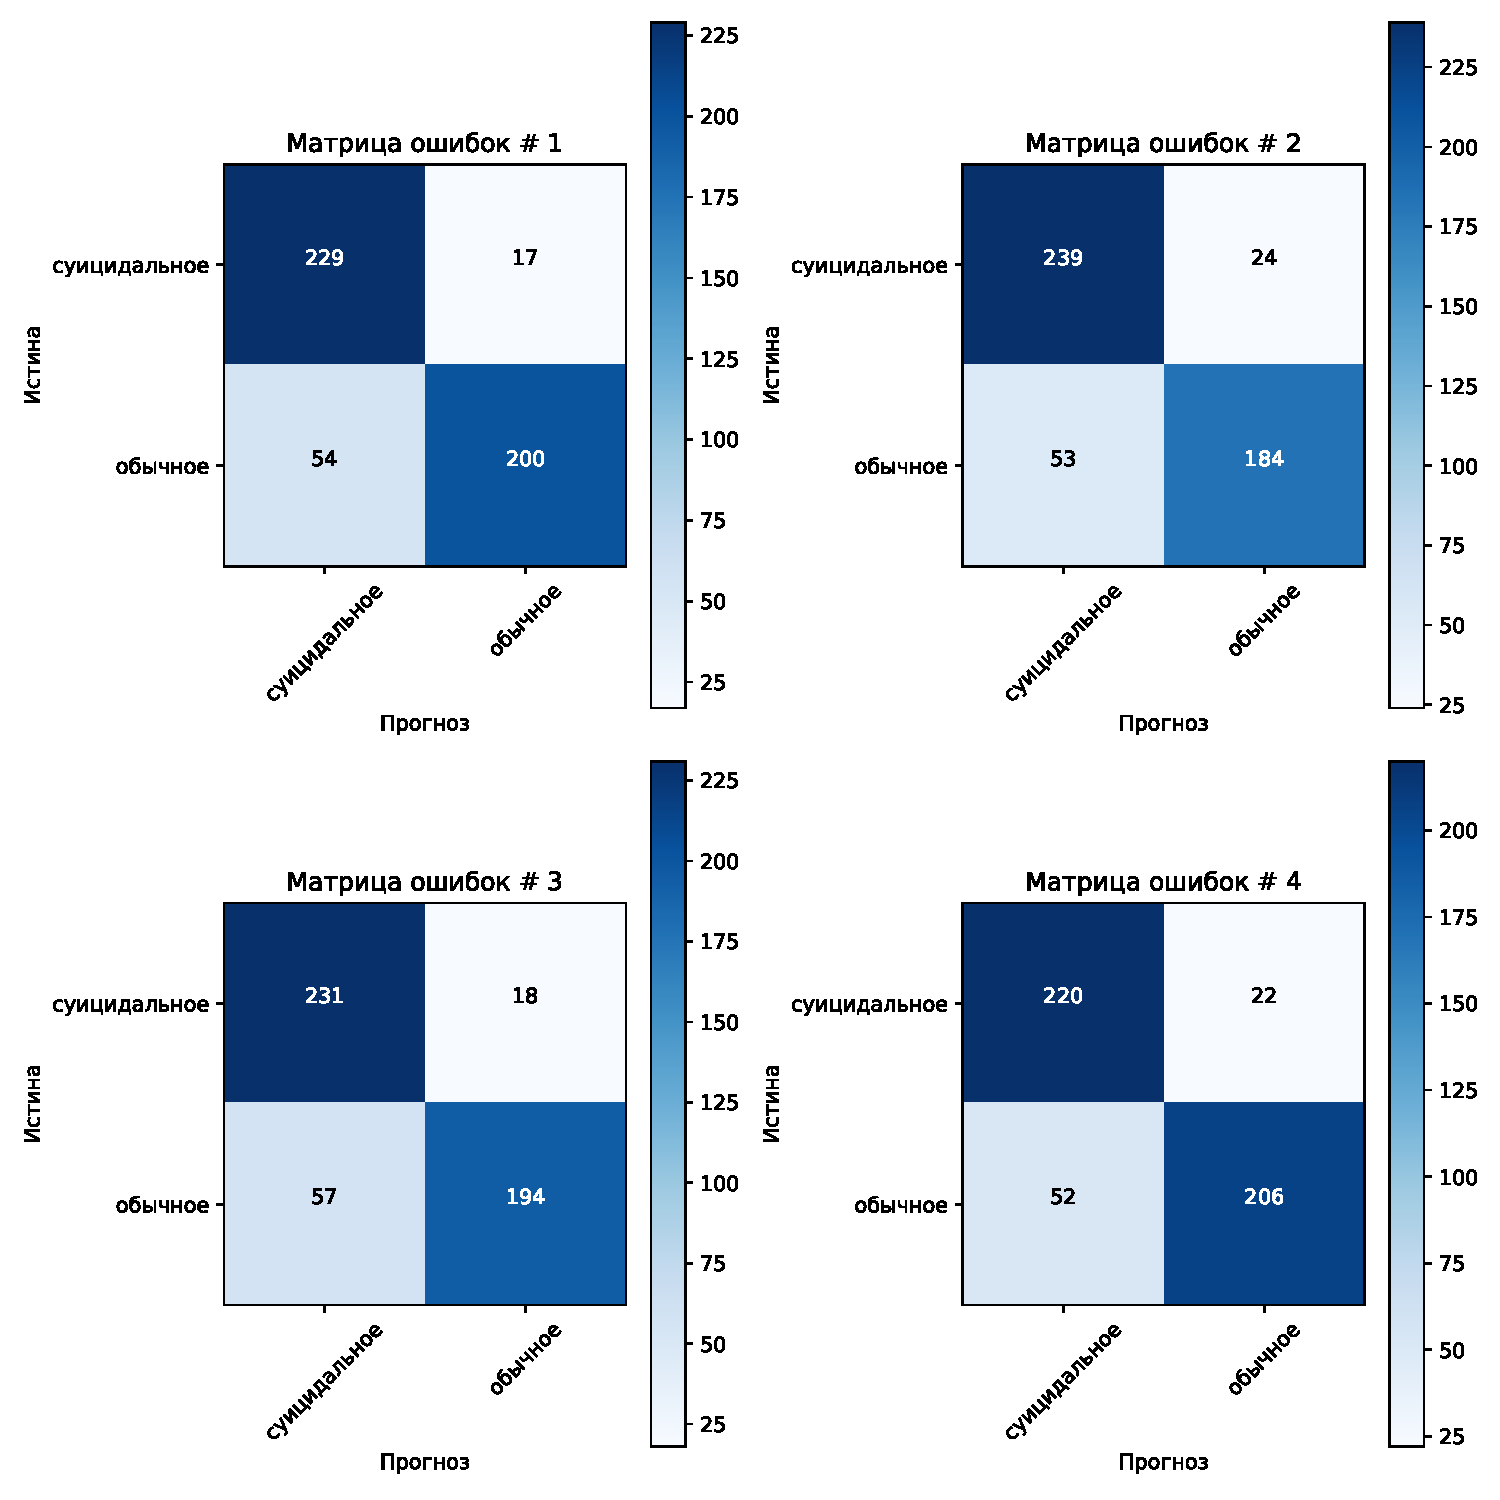
\includegraphics[width=\textwidth]{inc/plots/gradientMatrBag.pdf}
	\caption{ Матрицы ошибок в зависимости от номера разбиения, полученные с использованием градиентного бустинга (метод векторизации -- ``мешок слов''). }
	\label{img:gradientMatrBag}
\end{figure}

На рисунке \ref{img:gradientMetricsBag} представлены оценки классификатора, полученные с использованием градиентного бустинга, метод векторизации -- ``мешок слов''.
\begin{figure}[H]
	\centering
	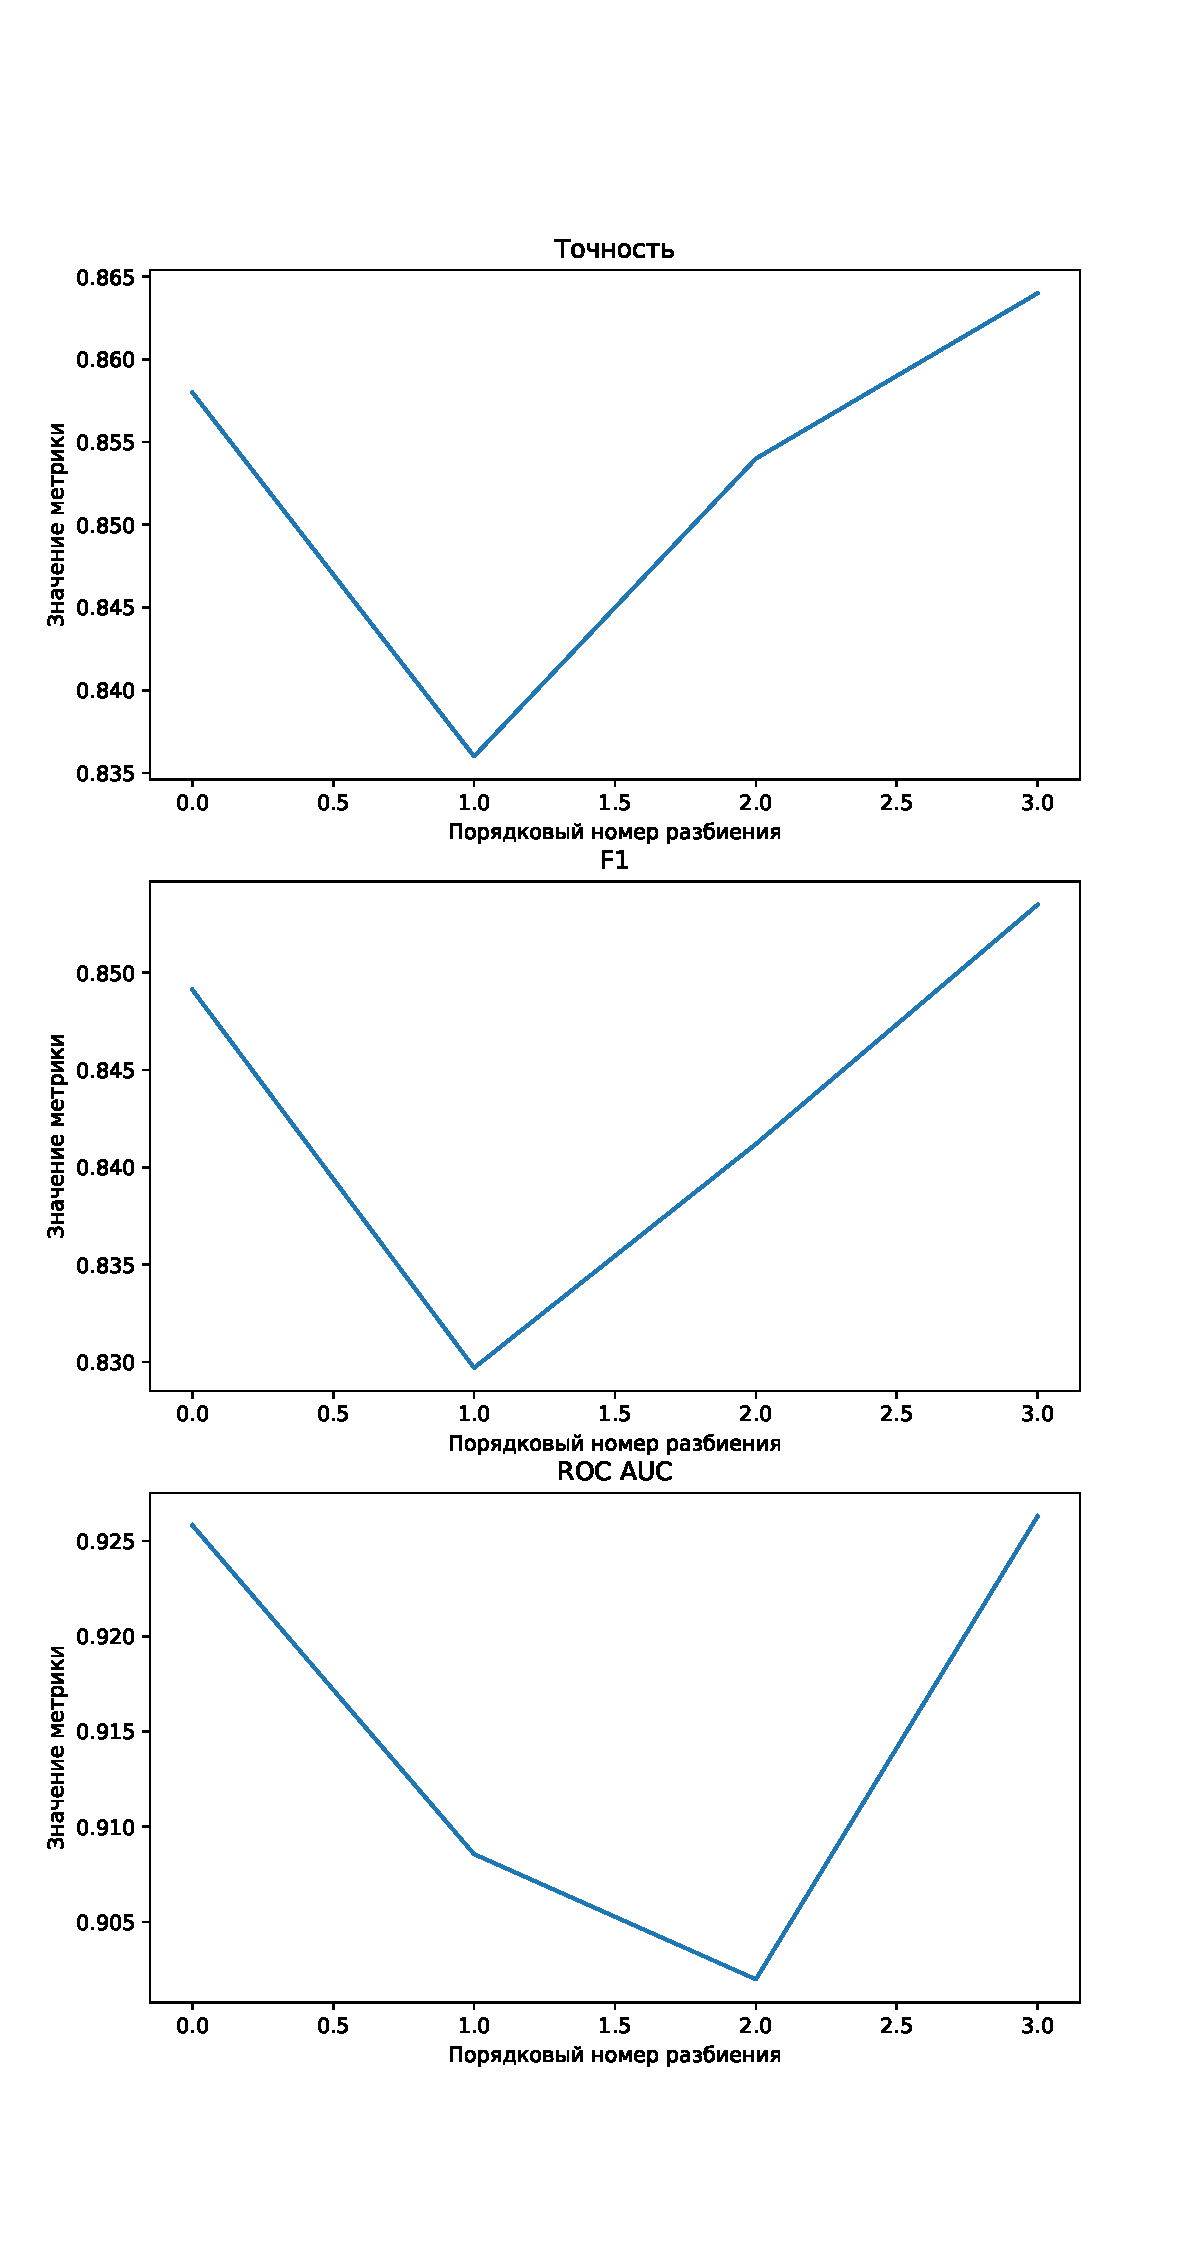
\includegraphics[height=23cm]{inc/plots/gradientMetricsBag.pdf}
	\caption{ Оценки классификатора в зависимости от номера разбиения, полученные с использованием градиентного бустинга (метод векторизации --  ``мешок слов''). }
	\label{img:gradientMetricsBag}
\end{figure}

Параметры модели при применении векторизации BERT:
\begin{itemize}
	\item скорость обучения -- ;
\end{itemize}

На рисунке \ref{img:gradientMatrBert} представлены матрицы ошибок, полученные с использованием градиентного бустинга, метод векторизации -- BERT.
\begin{figure}[H]
	\centering
	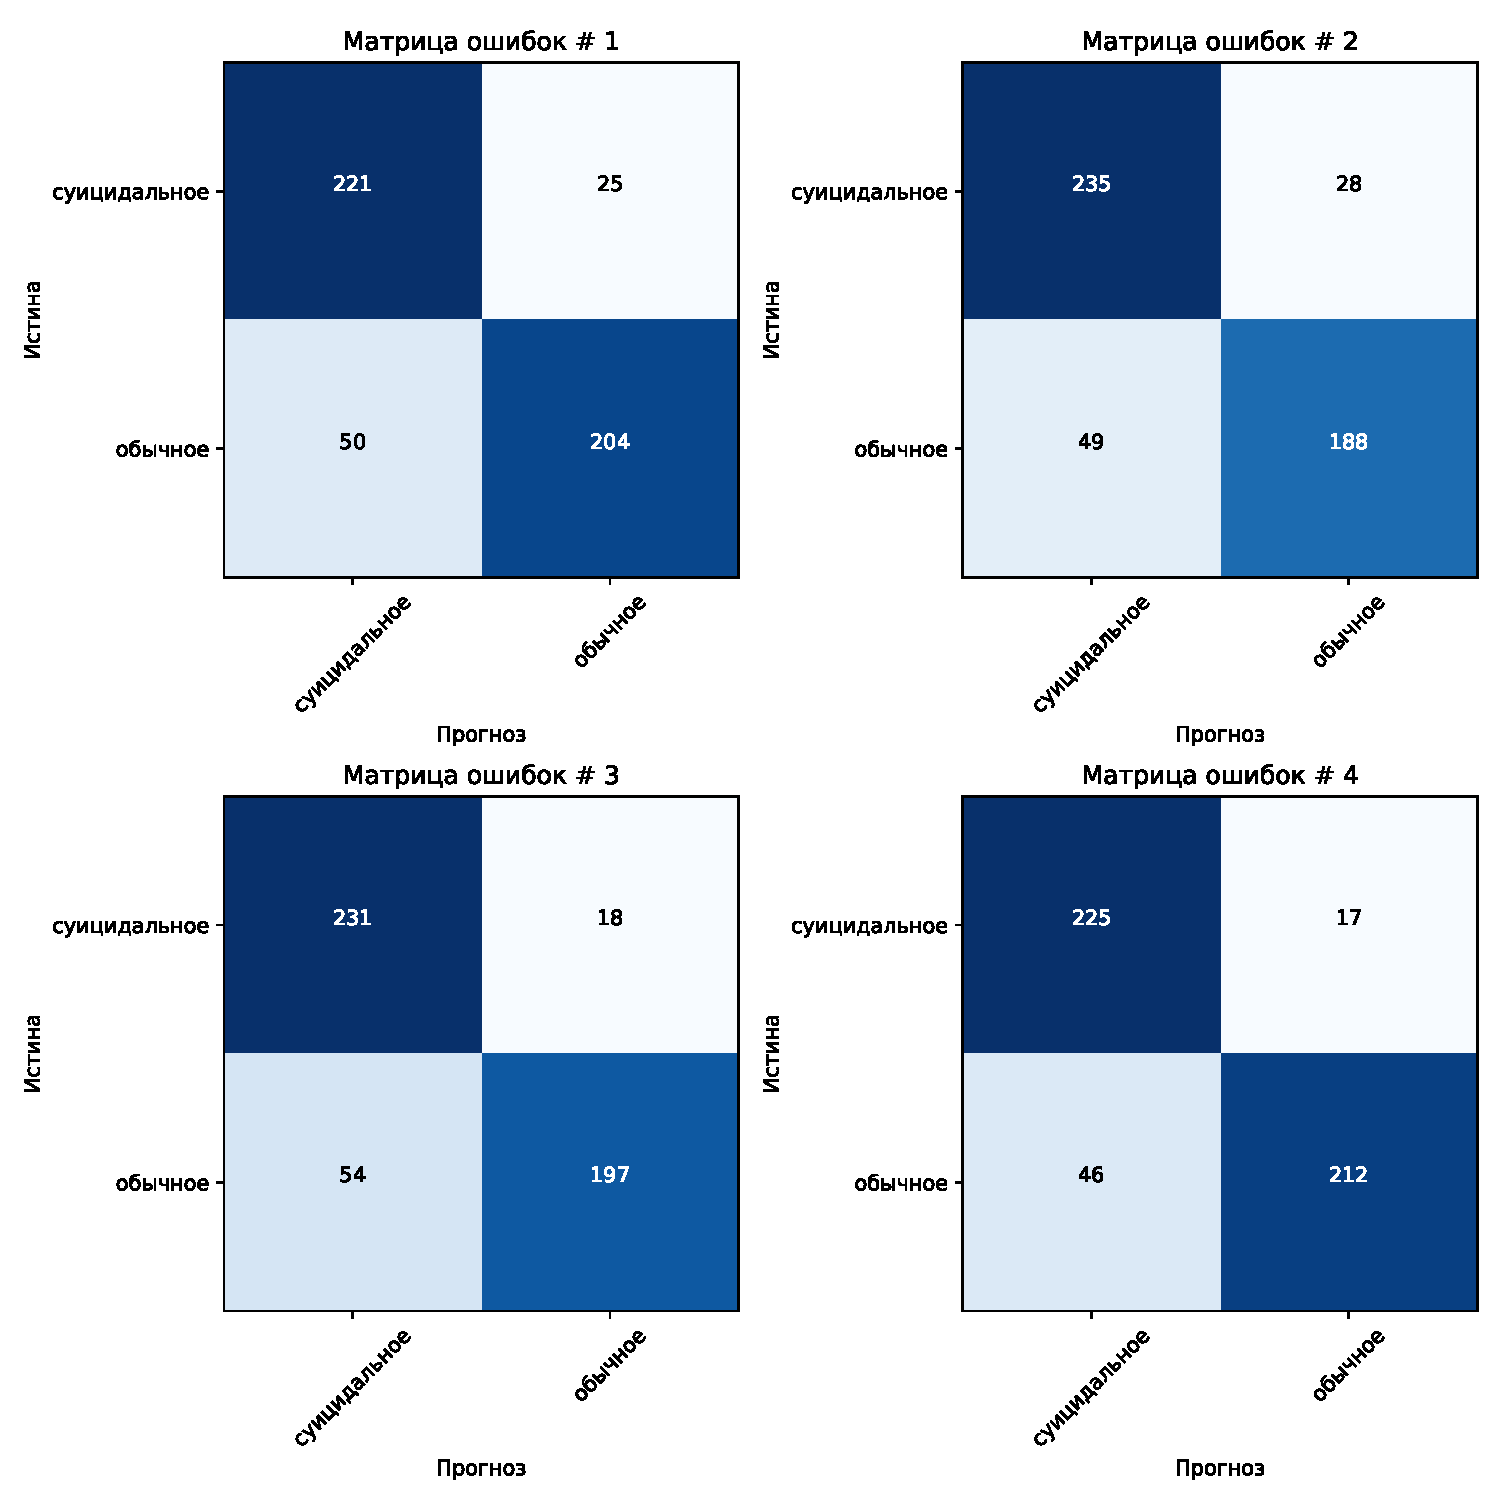
\includegraphics[width=\textwidth]{inc/plots/gradientMatrBert.pdf}
	\caption{ Матрицы ошибок в зависимости от номера разбиения, полученные с использованием градиентного бустинга (метод векторизации -- BERT). }
	\label{img:gradientMatrBert}
\end{figure}

На рисунке \ref{img:gradientMetricsBert} представлены оценки классификатора, полученные с использованием градиентного бустинга, метод векторизации -- BERT.
\begin{figure}[H]
	\centering
	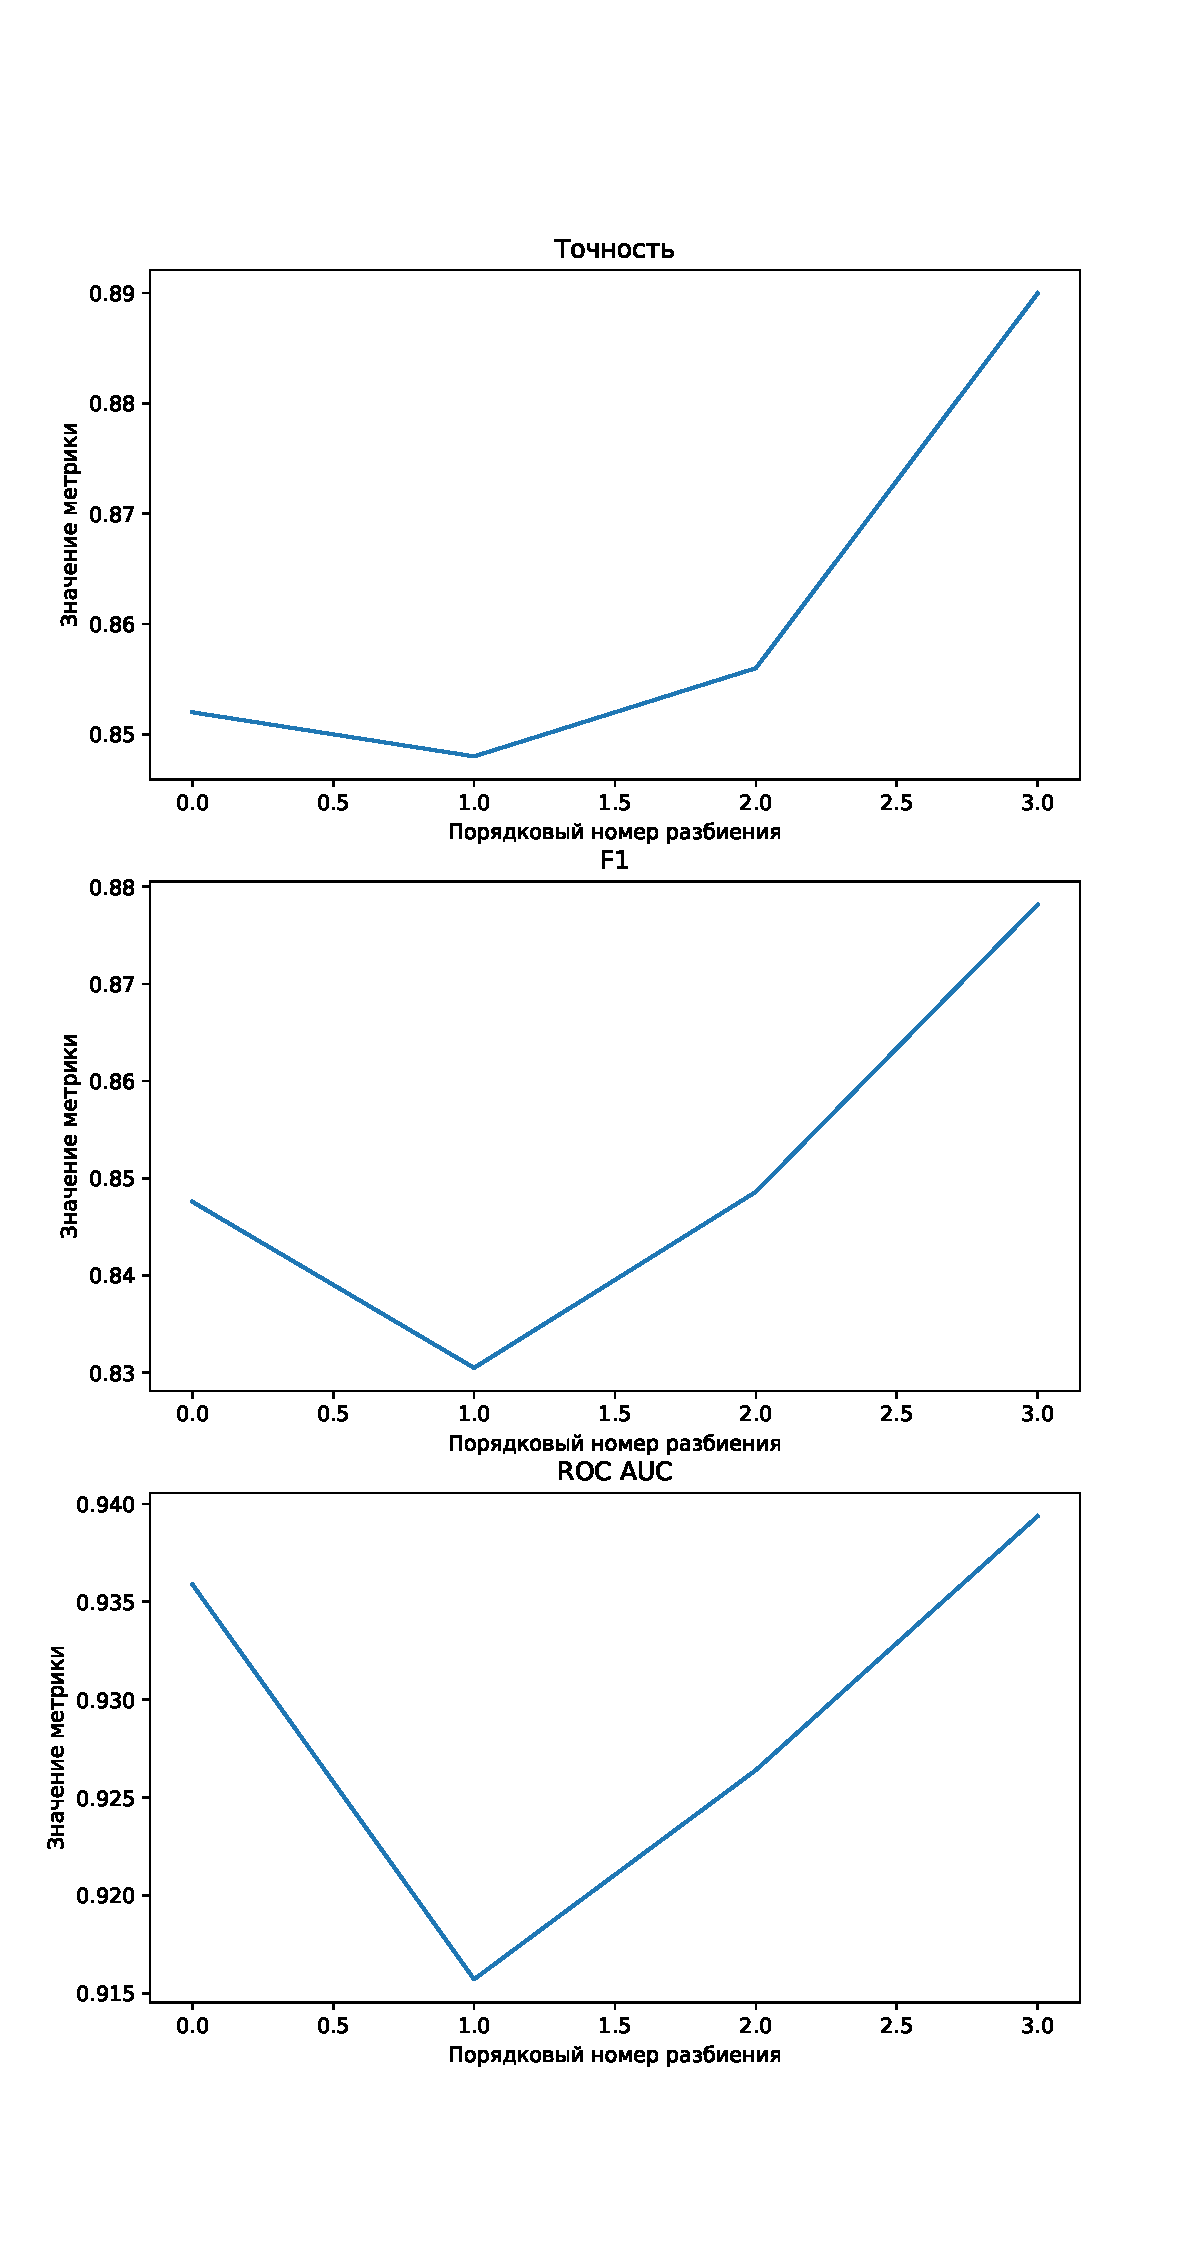
\includegraphics[height=23cm]{inc/plots/gradientMetricsBert.pdf}
	\caption{ Оценки классификатора в зависимости от номера разбиения, полученные с использованием градиентного бустинга (метод векторизации -- BERT). }
	\label{img:gradientMetricsBert}
\end{figure}



\subsection{ Метод случайного леса }

Параметры модели при применении метода векторизации ``мешок слов'':
\begin{itemize}
	\item скорость обучения -- ;
\end{itemize}

На рисунке \ref{img:randomMatrBag} представлены матрицы ошибок, полученные с использованием метода случайного леса, метод векторизации -- ``мешок слов''.
\begin{figure}[H]
	\centering
	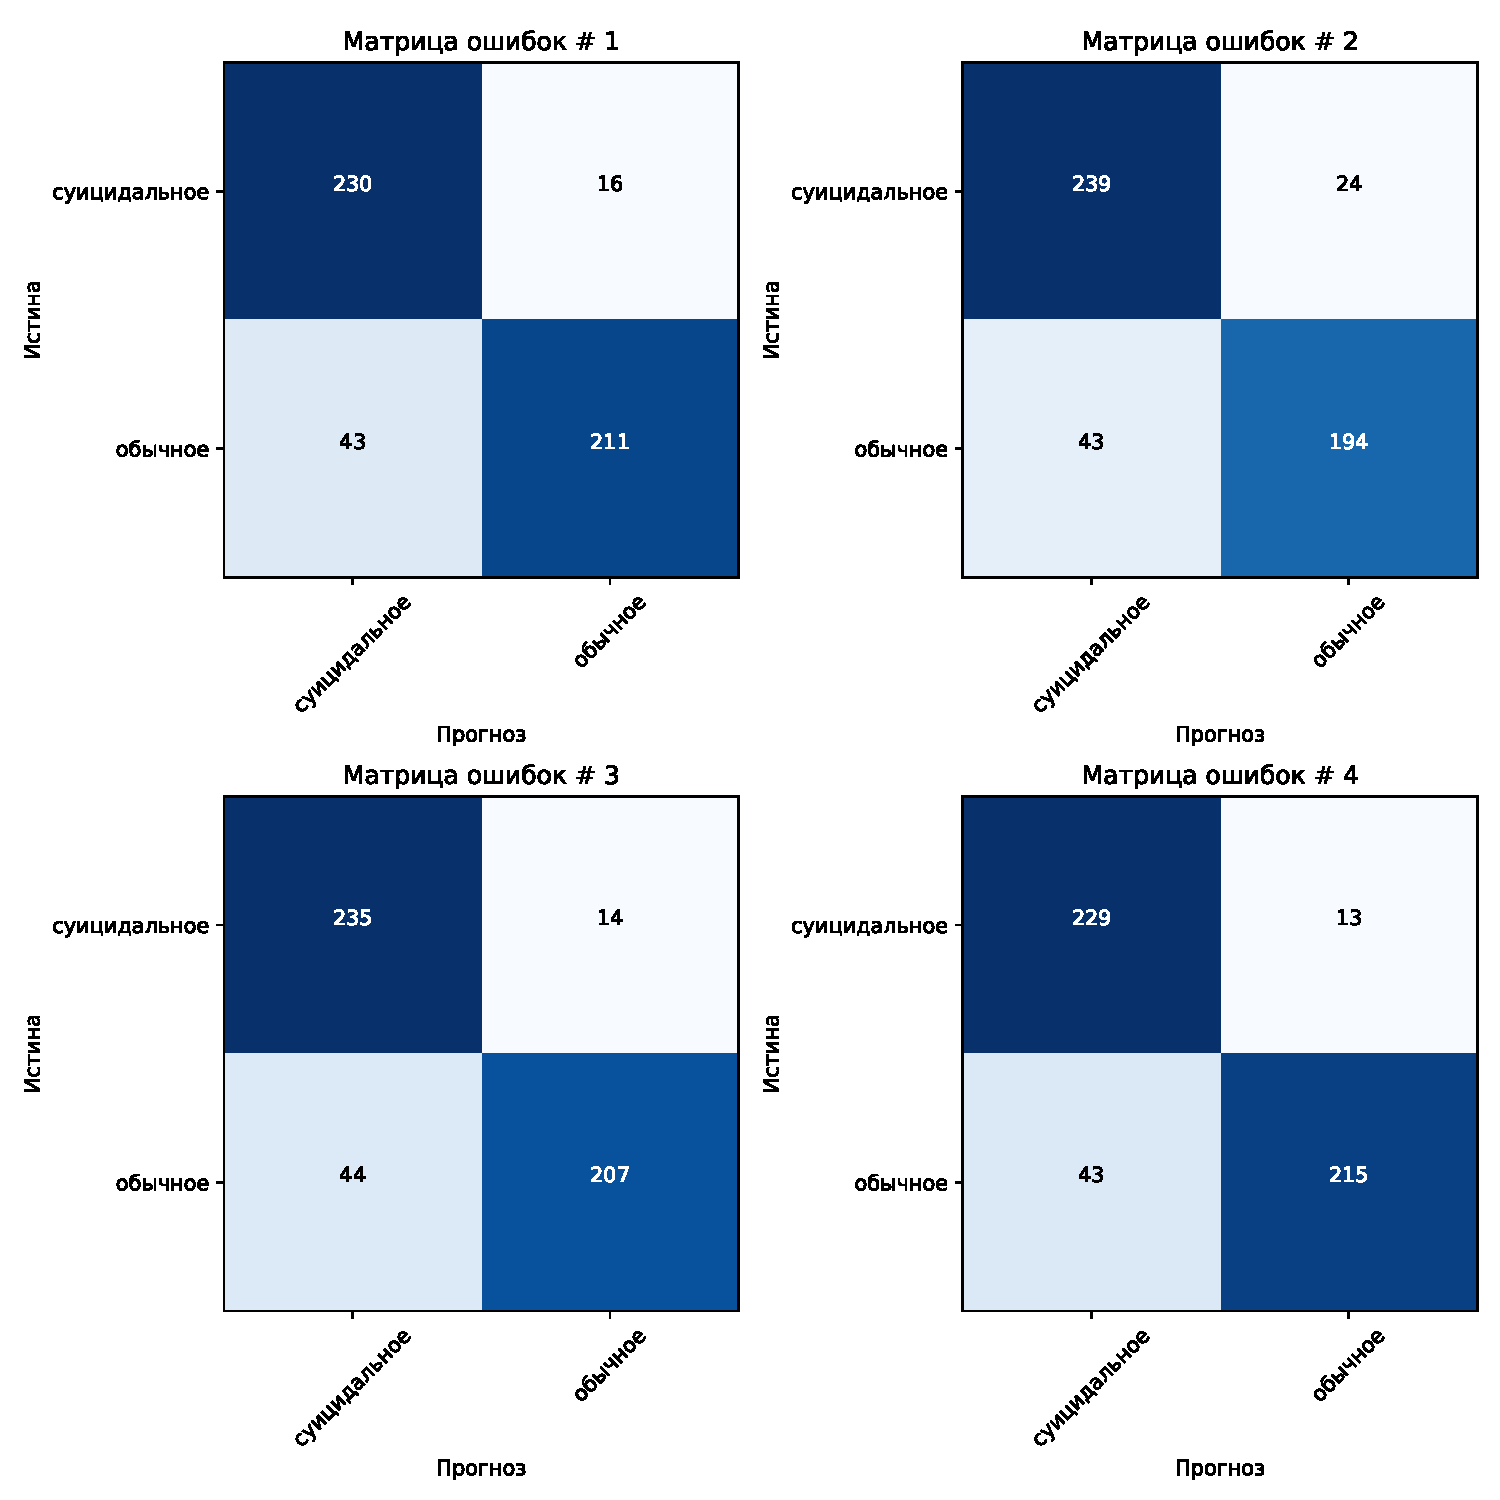
\includegraphics[width=\textwidth]{inc/plots/randomMatrBag.pdf}
	\caption{ Матрицы ошибок в зависимости от номера разбиения, полученные с использованием метода случайного леса (метод векторизации -- ``мешок слов''). }
	\label{img:randomMatrBag}
\end{figure}

На рисунке \ref{img:randomMetricsBag} представлены оценки классификатора, полученные с использованием метода случайного леса, метод векторизации -- ``мешок слов''.
\begin{figure}[H]
	\centering
	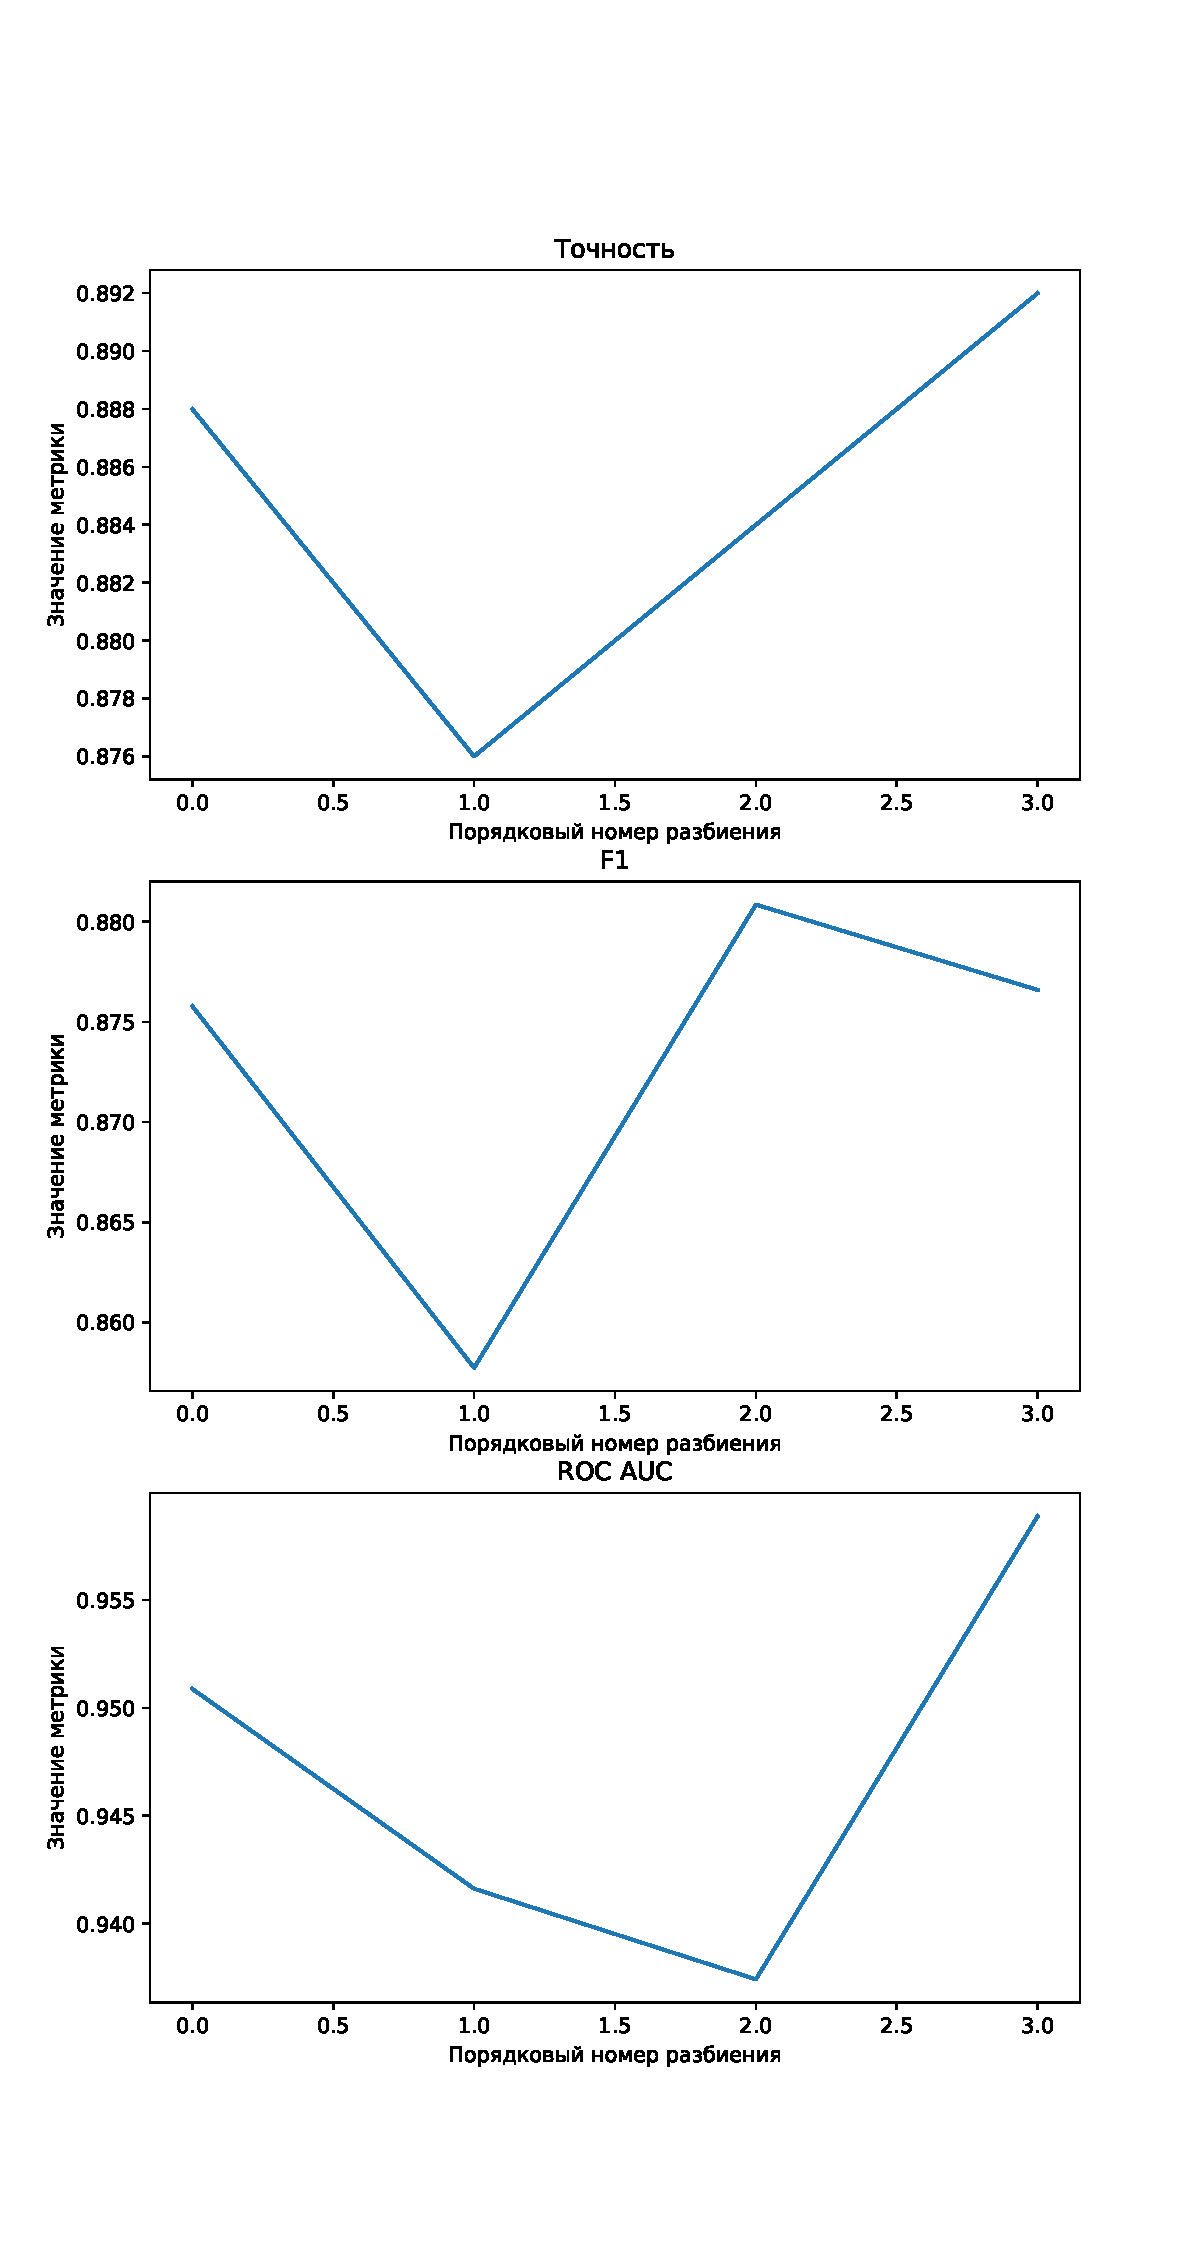
\includegraphics[height=23cm]{inc/plots/randomMetricsBag.pdf}
	\caption{ Оценки классификатора в зависимости от номера разбиения, полученные с использованием метода случайного леса (метод векторизации --  ``мешок слов''). }
	\label{img:randomMetricsBag}
\end{figure}


Параметры модели при применении векторизации BERT:
\begin{itemize}
	\item скорость обучения -- ;
\end{itemize}

На рисунке \ref{img:randomMatrBert} представлены матрицы ошибок, полученные с использованием метода случайного леса, метод векторизации -- BERT.
\begin{figure}[H]
	\centering
	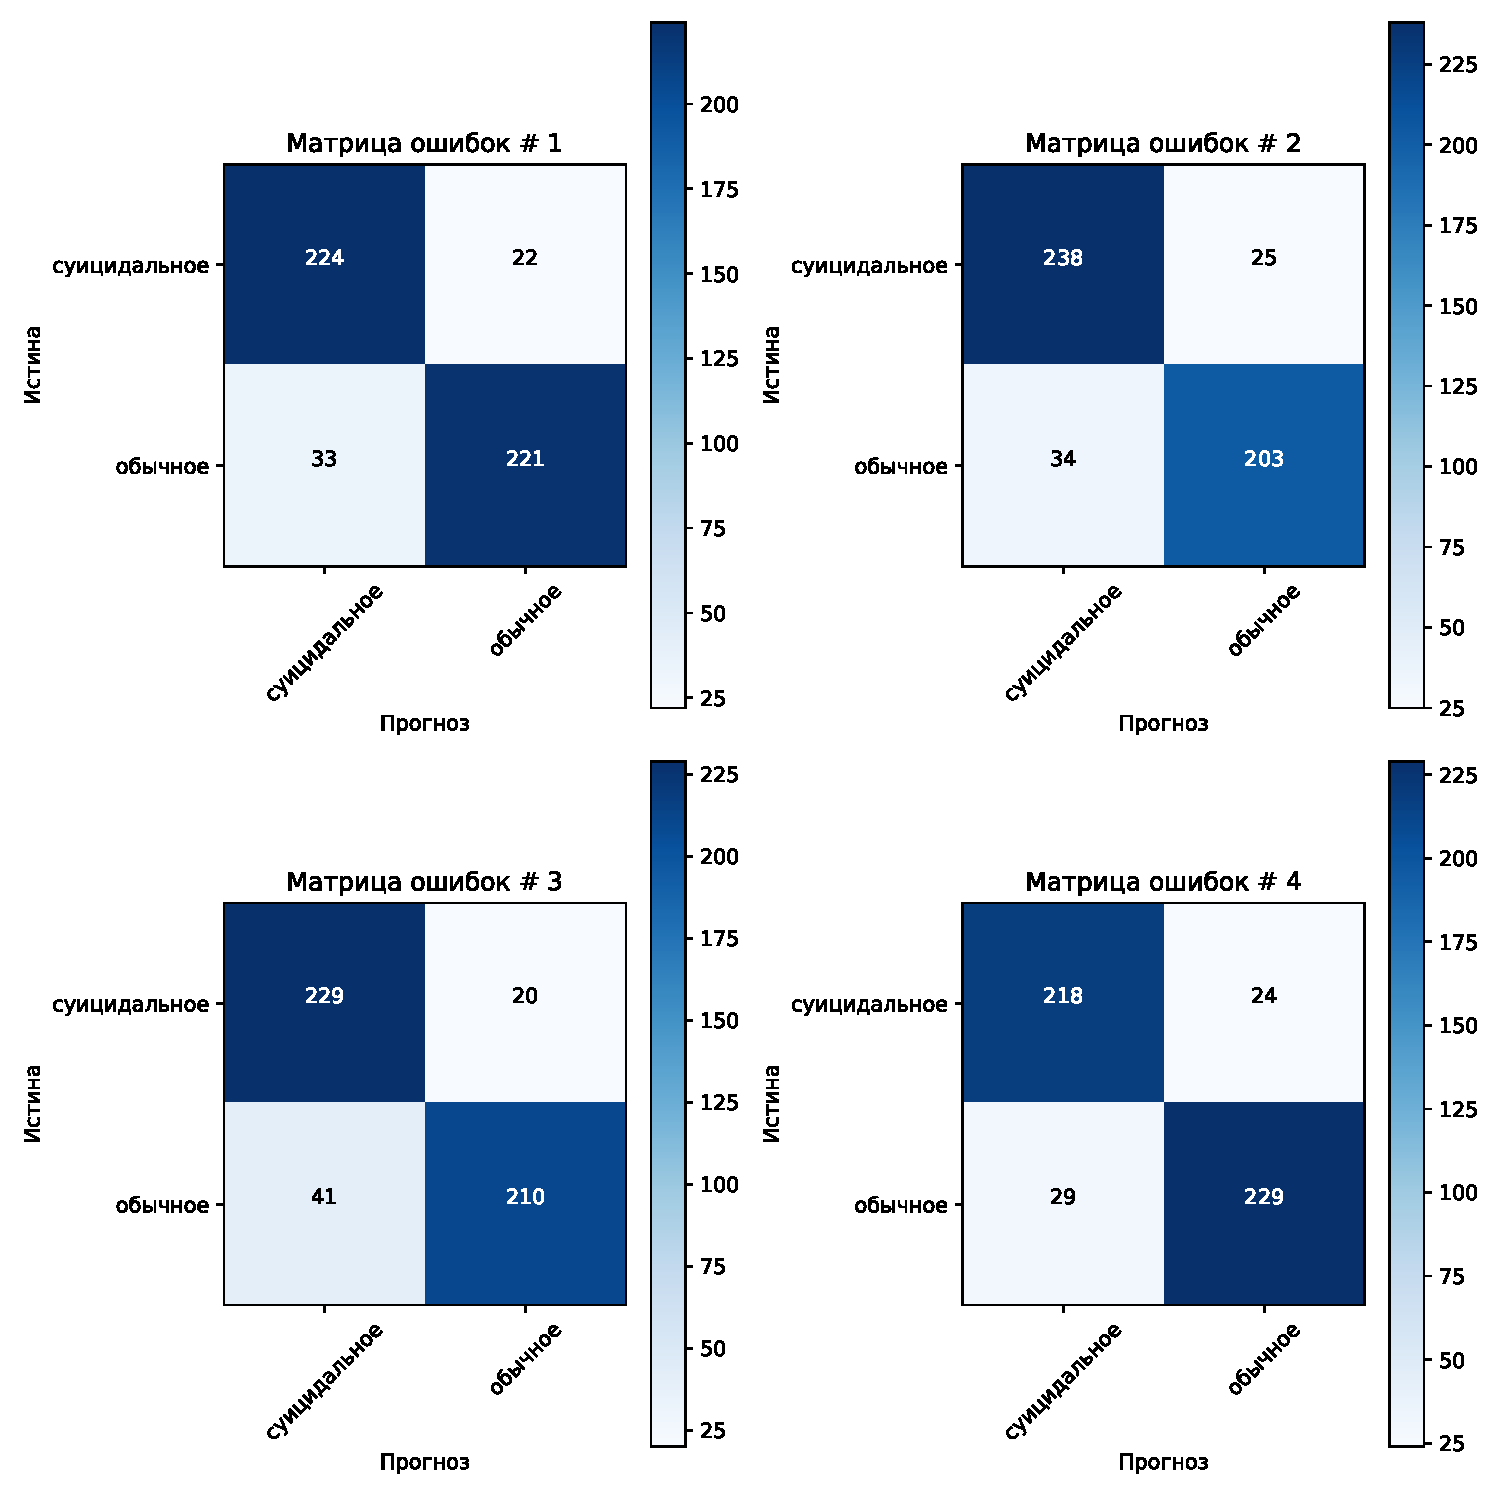
\includegraphics[width=\textwidth]{inc/plots/randomMatrBert.pdf}
	\caption{ Матрицы ошибок в зависимости от номера разбиения, полученные с использованием метода случайного леса (метод векторизации -- BERT). }
	\label{img:randomMatrBert}
\end{figure}

На рисунке \ref{img:randomMetricsBert} представлены оценки классификатора, полученные с использованием метода случайного леса, метод векторизации -- BERT.
\begin{figure}[H]
	\centering
	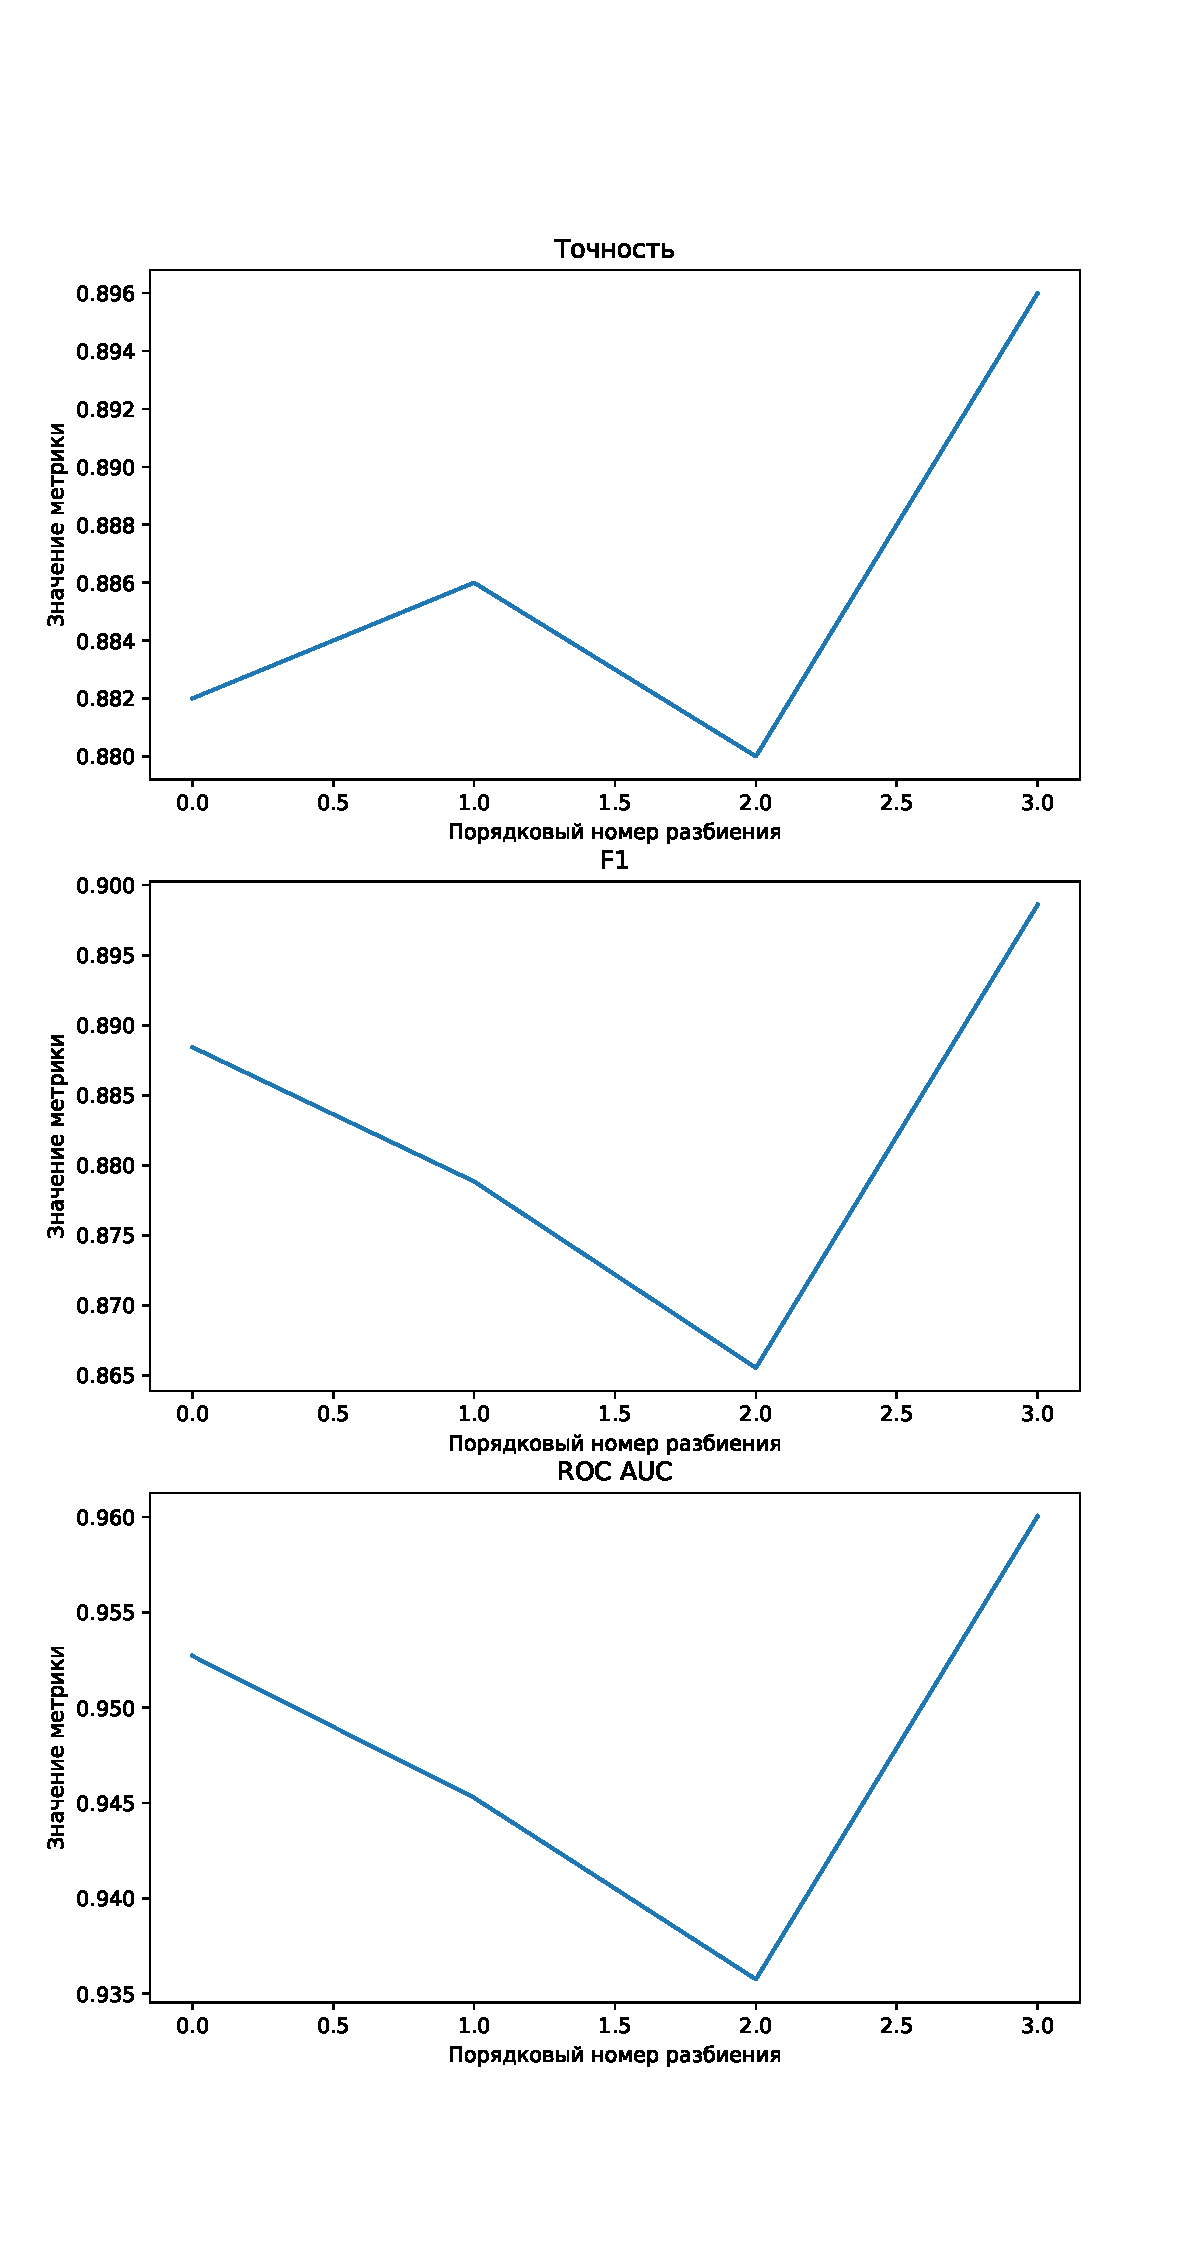
\includegraphics[height=23cm]{inc/plots/randomMetricsBert.pdf}
	\caption{ Оценки классификатора в зависимости от номера разбиения, полученные с использованием метода случайного леса (метод векторизации -- BERT). }
	\label{img:randomMetricsBert}
\end{figure}



\subsection{ Метод опорных векторов }

Параметры модели при применении метода векторизации ``мешок слов'':
\begin{itemize}
	\item скорость обучения -- ;
\end{itemize}

На рисунке \ref{img:svcMatrBag} представлены матрицы ошибок, полученные с использованием метода опорных векторов, метод векторизации -- ``мешок слов''.
\begin{figure}[H]
	\centering
	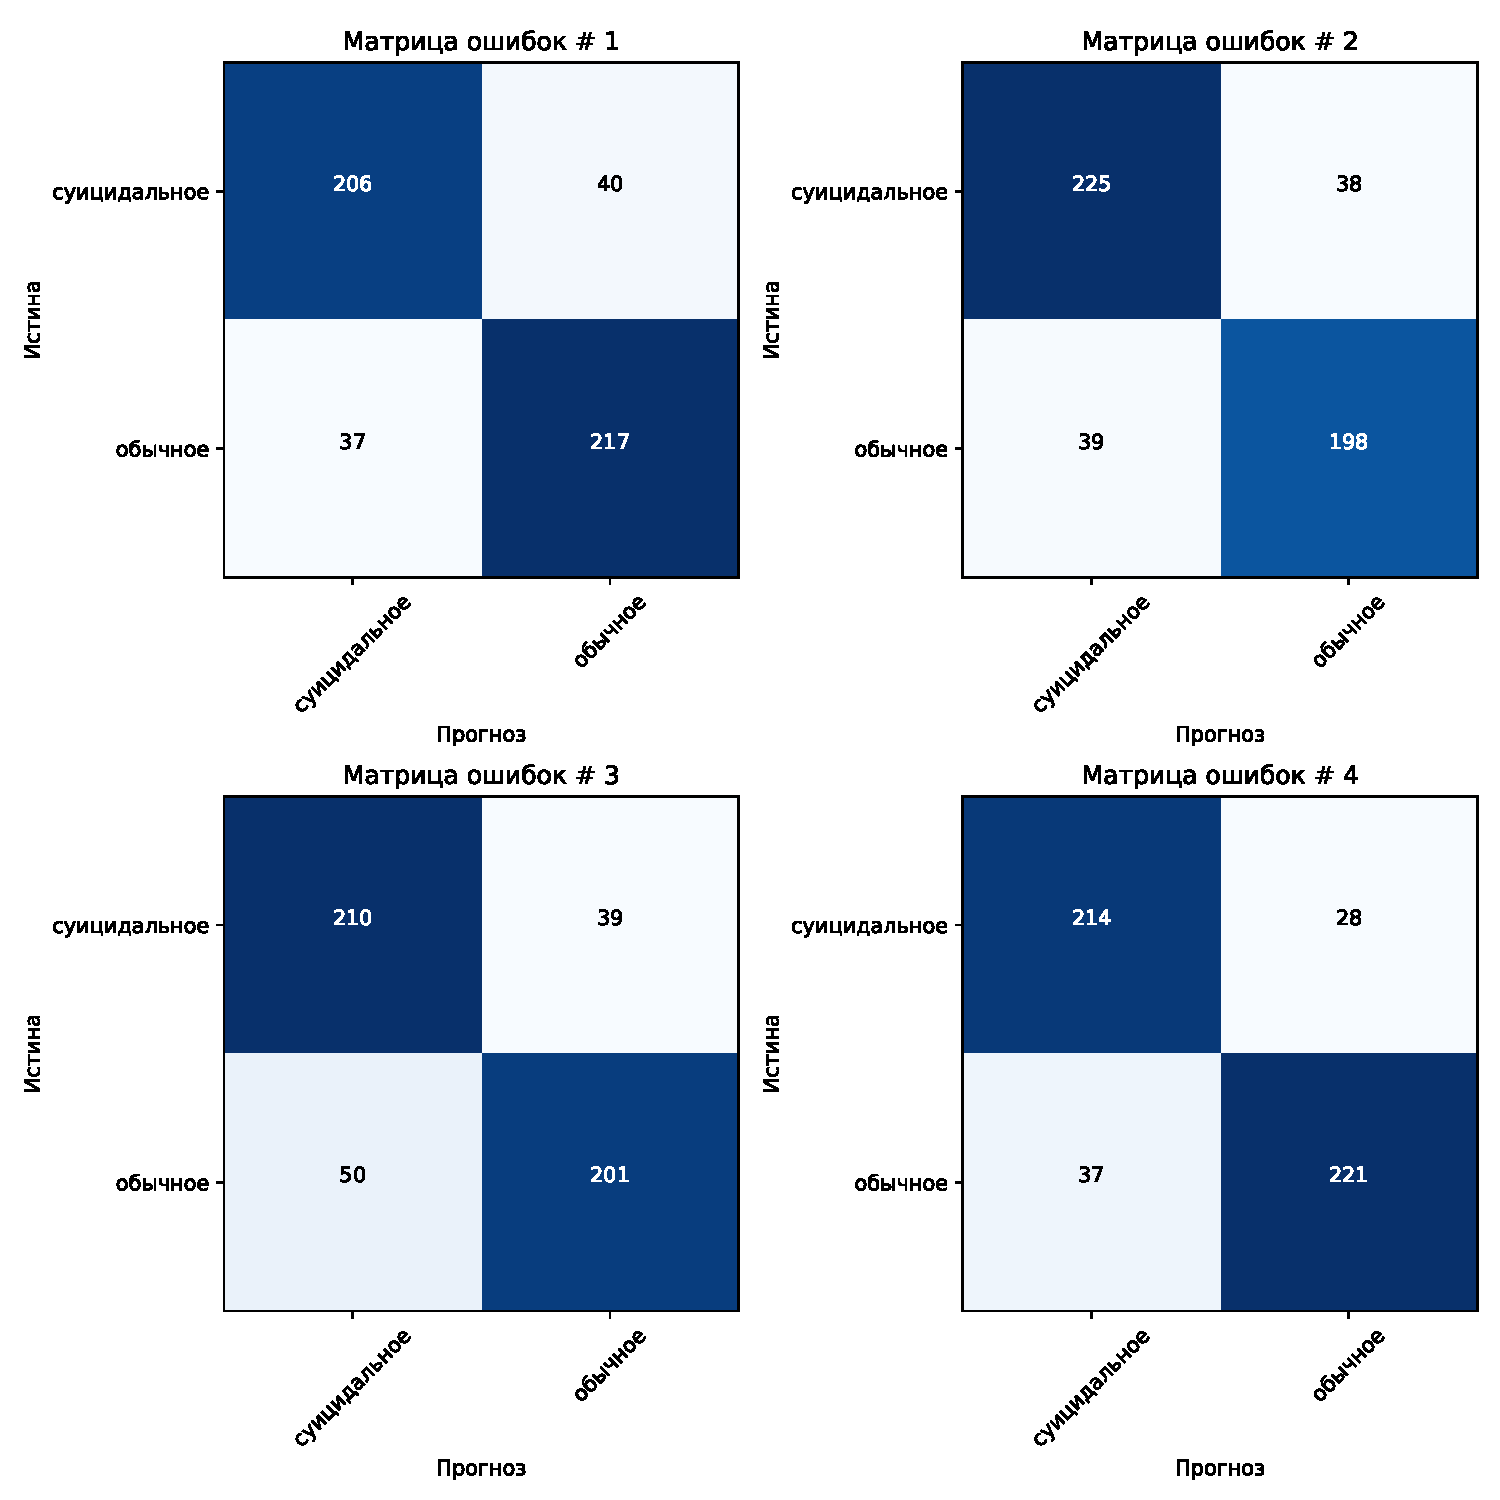
\includegraphics[width=\textwidth]{inc/plots/svcMatrBag.pdf}
	\caption{ Матрицы ошибок в зависимости от номера разбиения, полученные с использованием метода опорных векторов (метод векторизации -- ``мешок слов''). }
	\label{img:svcMatrBag}
\end{figure}

На рисунке \ref{img:svcMetricsBag} представлены оценки классификатора, полученные с использованием метода опорных векторов, метод векторизации -- ``мешок слов''.
\begin{figure}[H]
	\centering
	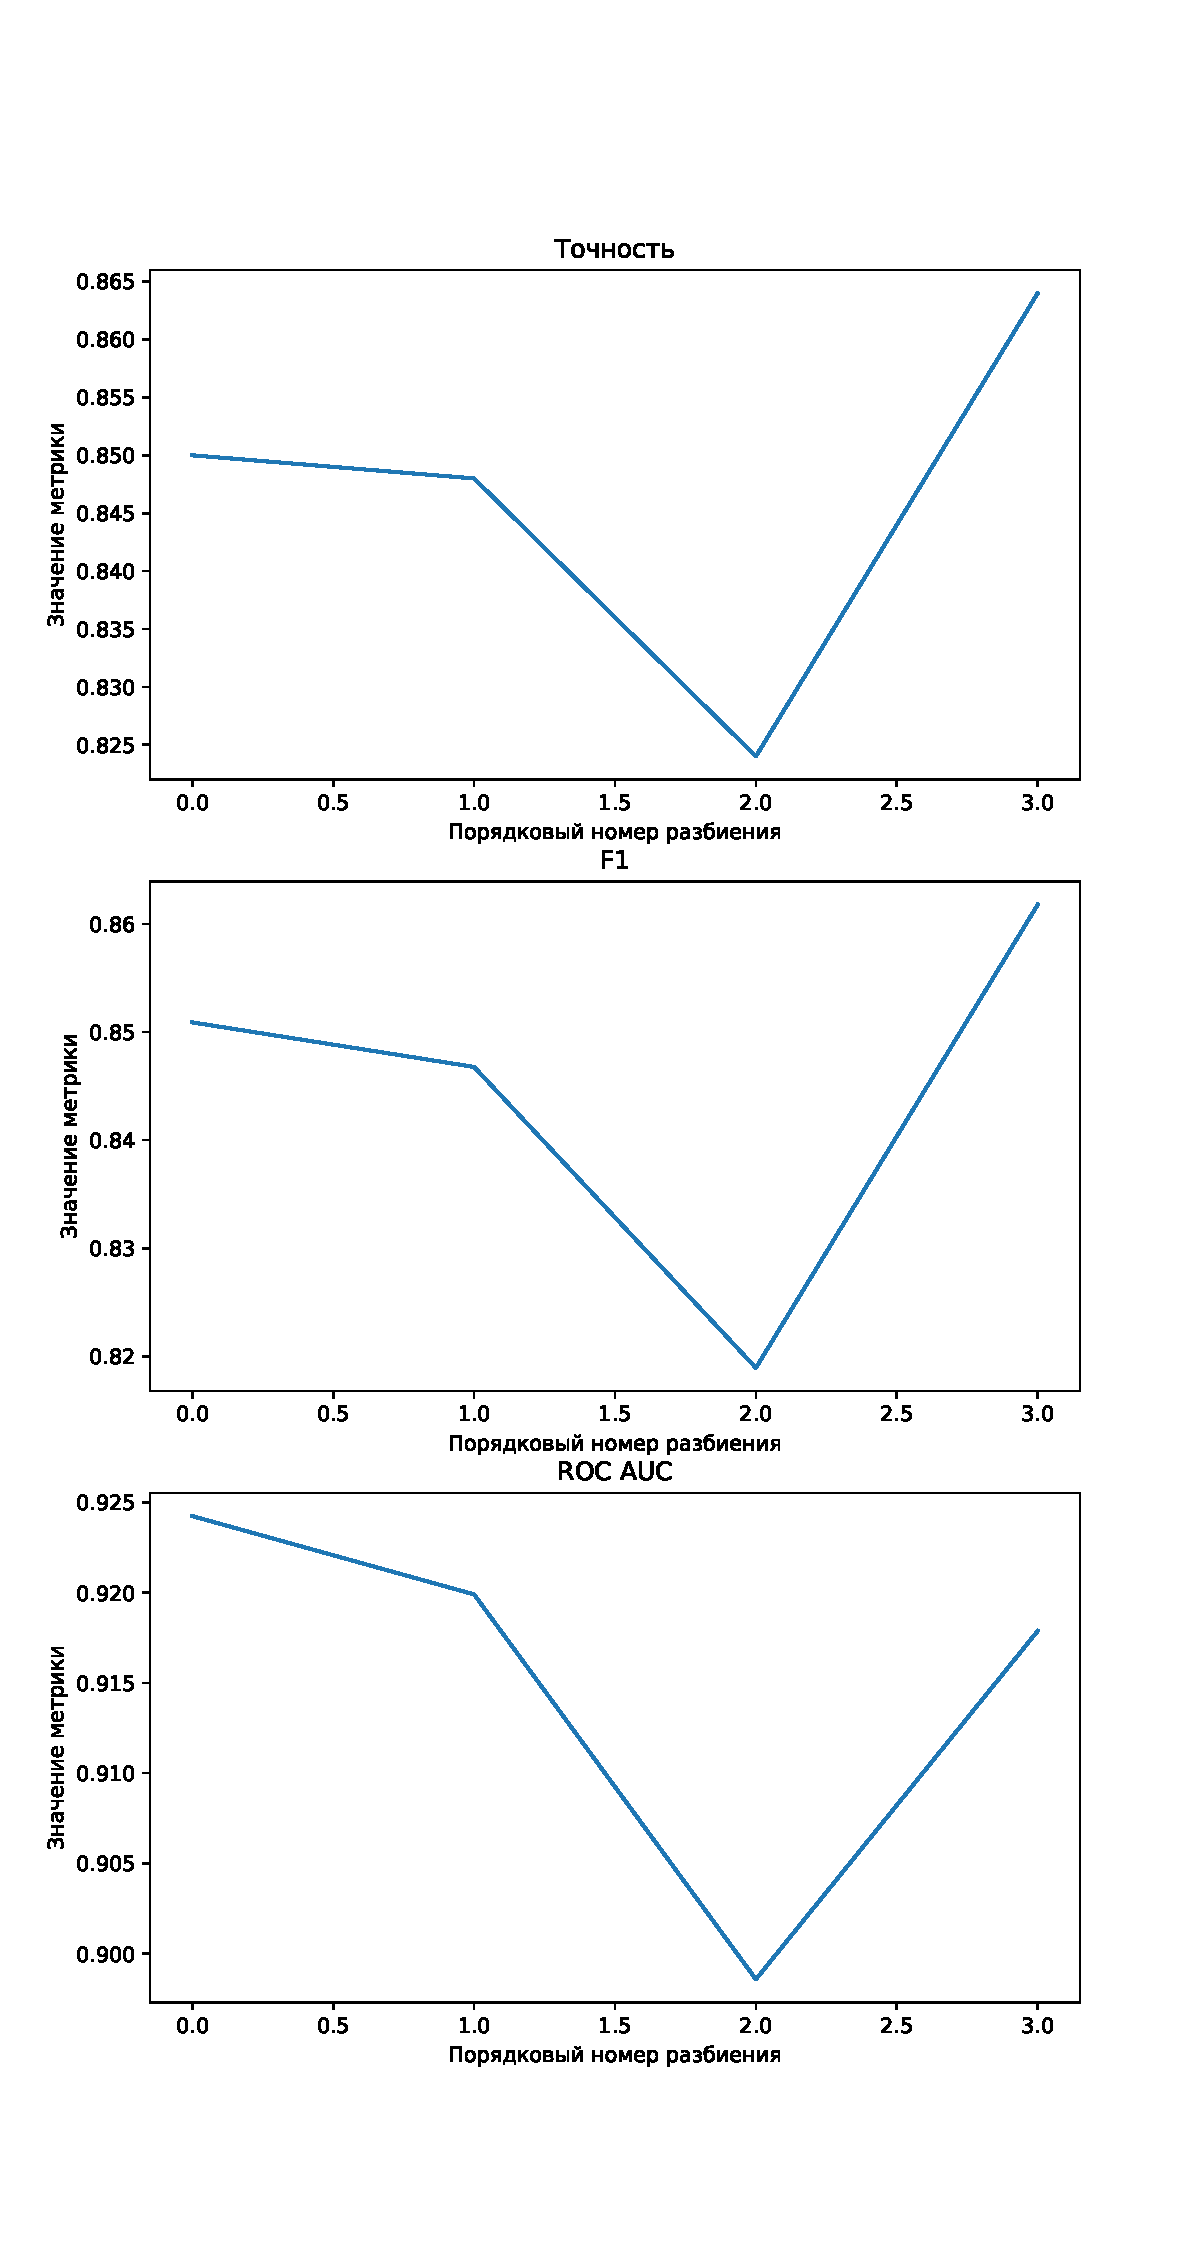
\includegraphics[height=23cm]{inc/plots/svcMetricsBag.pdf}
	\caption{ Оценки классификатора в зависимости от номера разбиения, полученные с использованием метода опорных векторов (метод векторизации --  ``мешок слов''). }
	\label{img:svcMetricsBag}
\end{figure}


Параметры модели при применении векторизации BERT:
\begin{itemize}
	\item скорость обучения -- ;
\end{itemize}

На рисунке \ref{img:svcMatrBert} представлены матрицы ошибок, полученные с использованием метода опорных векторов, метод векторизации -- BERT.
\begin{figure}[H]
	\centering
	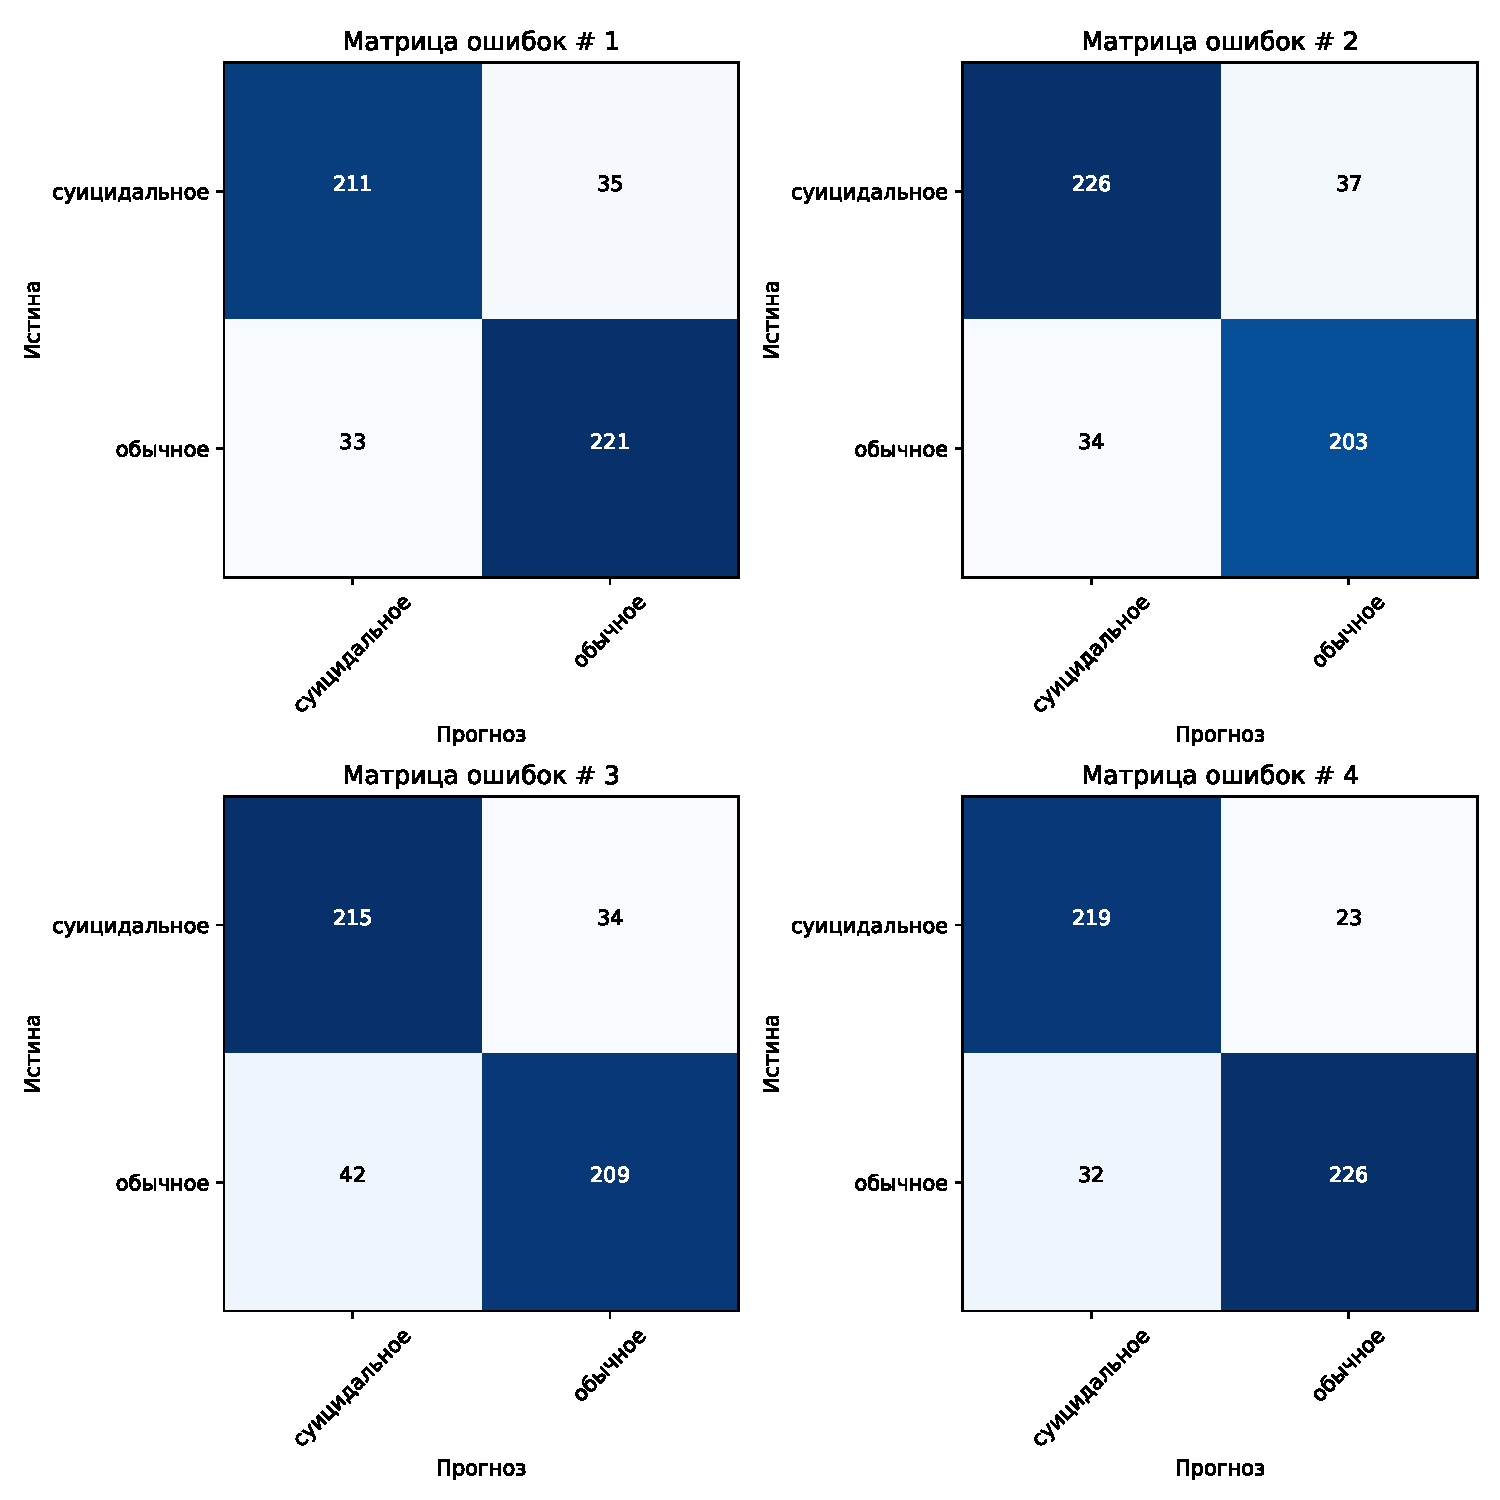
\includegraphics[width=\textwidth]{inc/plots/svcMatrBert.pdf}
	\caption{ Матрицы ошибок в зависимости от номера разбиения, полученные с использованием метода опорных векторов (метод векторизации -- BERT). }
	\label{img:svcMatrBert}
\end{figure}

На рисунке \ref{img:svcMetricsBert} представлены оценки классификатора, полученные с использованием метода опорных векторов, метод векторизации -- BERT.
\begin{figure}[H]
	\centering
	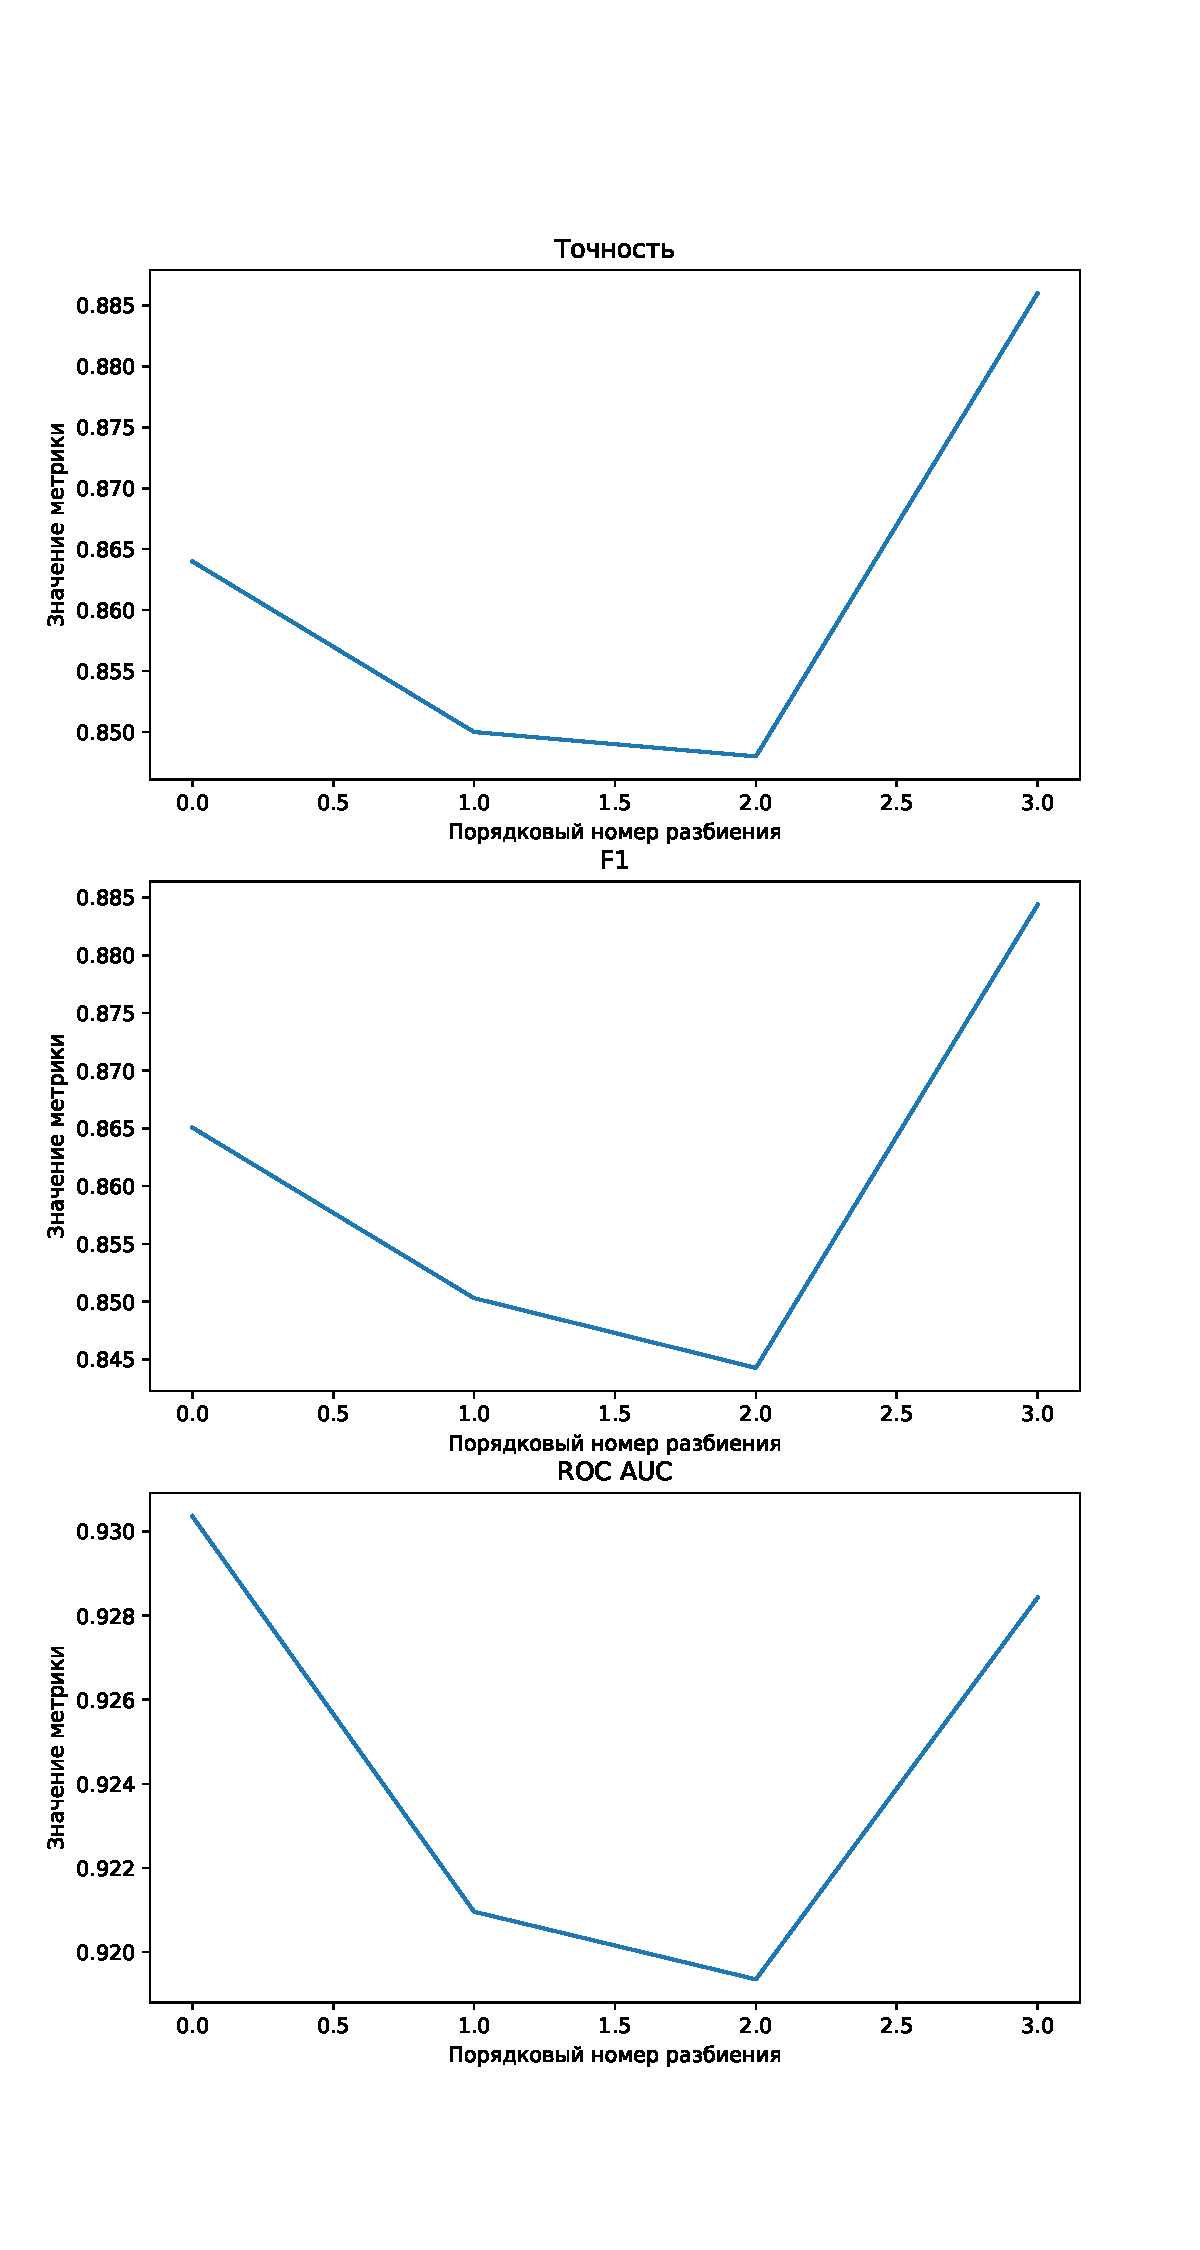
\includegraphics[height=23cm]{inc/plots/svcMetricsBert.pdf}
	\caption{ Оценки классификатора в зависимости от номера разбиения, полученные с использованием метода опорных векторов (метод векторизации -- BERT). }
	\label{img:svcMetricsBert}
\end{figure}



\subsection{ Метод K-ближайших соседей }

Параметры модели при применении метода векторизации ``мешок слов'':
\begin{itemize}
	\item скорость обучения -- ;
\end{itemize}

На рисунке \ref{img:knnMatrBag} представлены матрицы ошибок, полученные с использованием метода K-ближайших соседей, метод векторизации -- ``мешок слов''.
\begin{figure}[H]
	\centering
	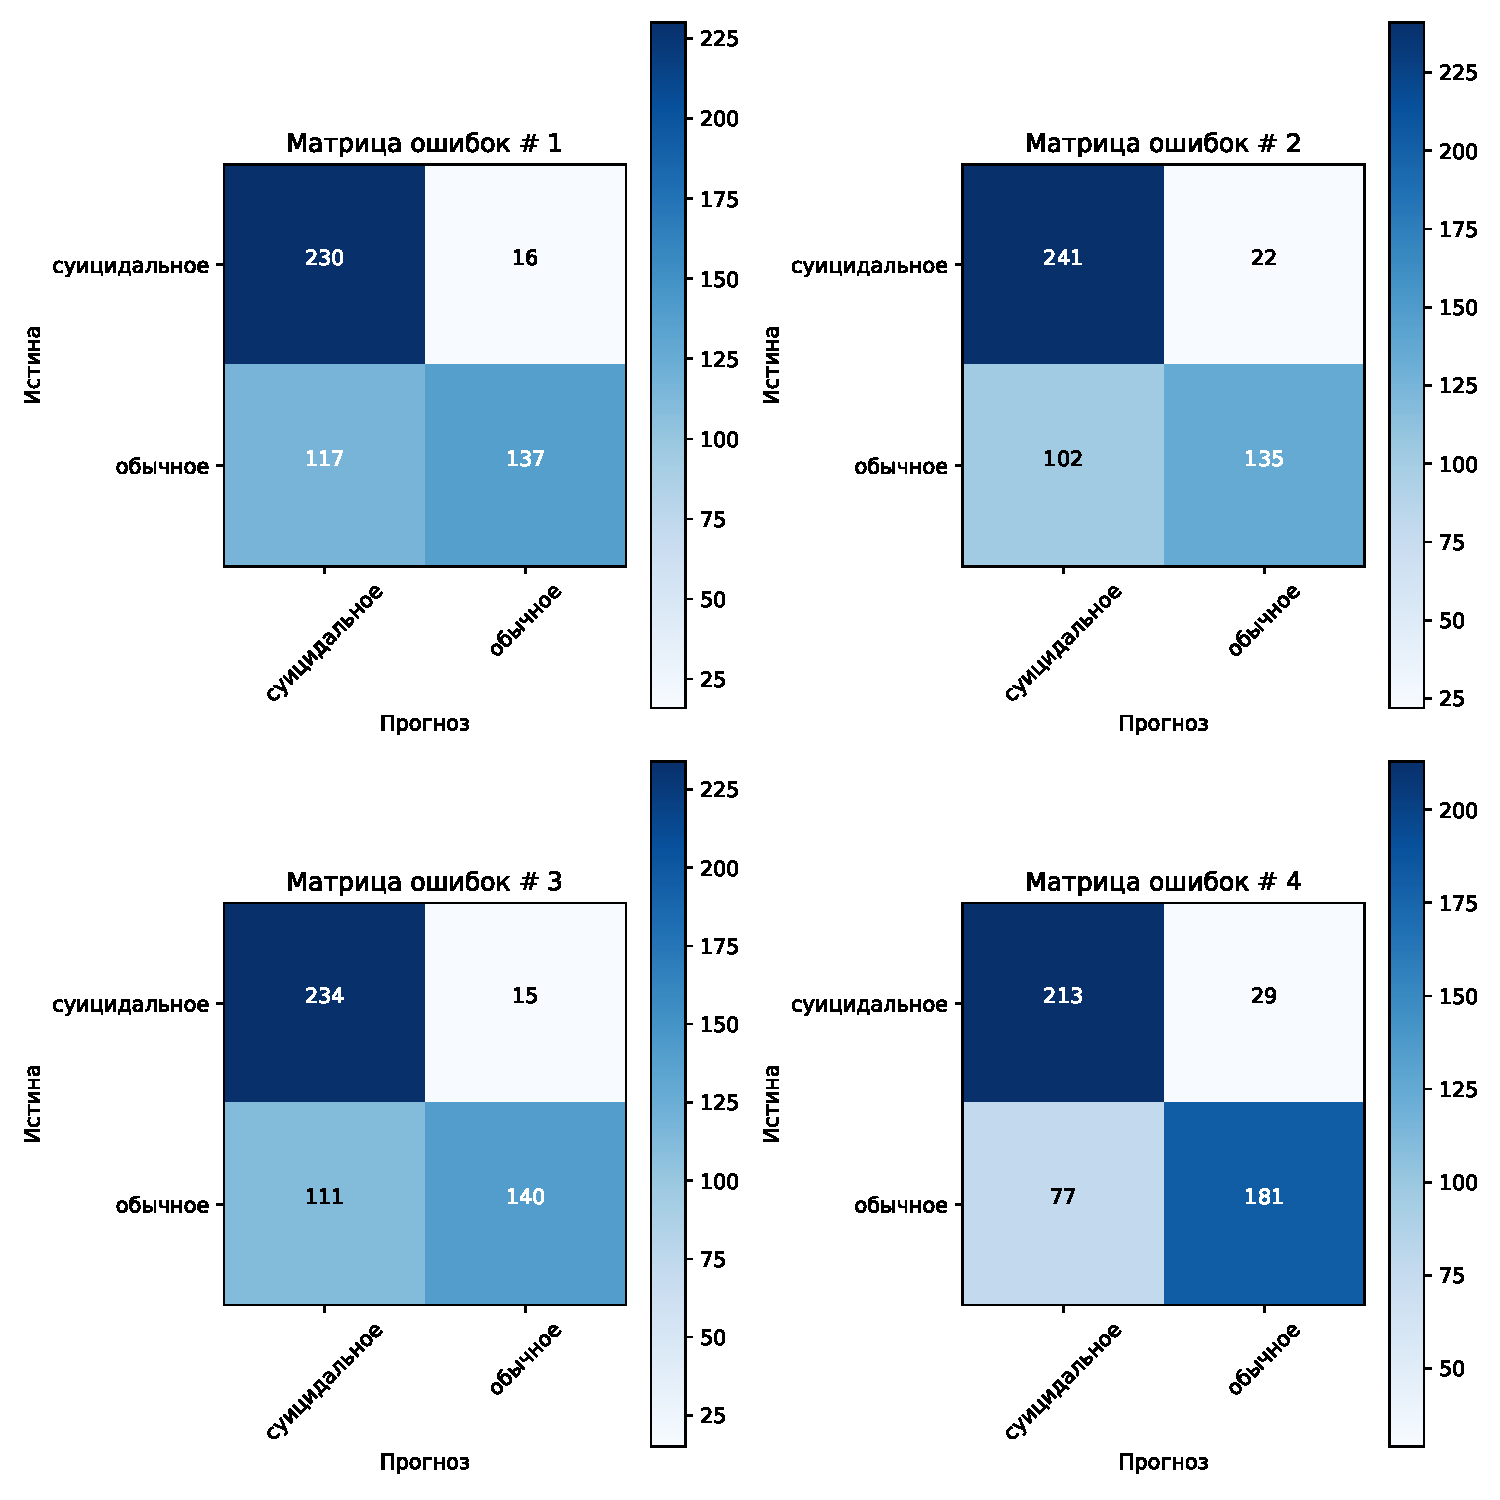
\includegraphics[width=\textwidth]{inc/plots/knnMatrBag.pdf}
	\caption{ Матрицы ошибок в зависимости от номера разбиения, полученные с использованием метода K-ближайших соседей (метод векторизации -- ``мешок слов''). }
	\label{img:knnMatrBag}
\end{figure}

На рисунке \ref{img:knnMetricsBag} представлены оценки классификатора, полученные с использованием метода K-ближайших соседей, метод векторизации -- ``мешок слов''.
\begin{figure}[H]
	\centering
	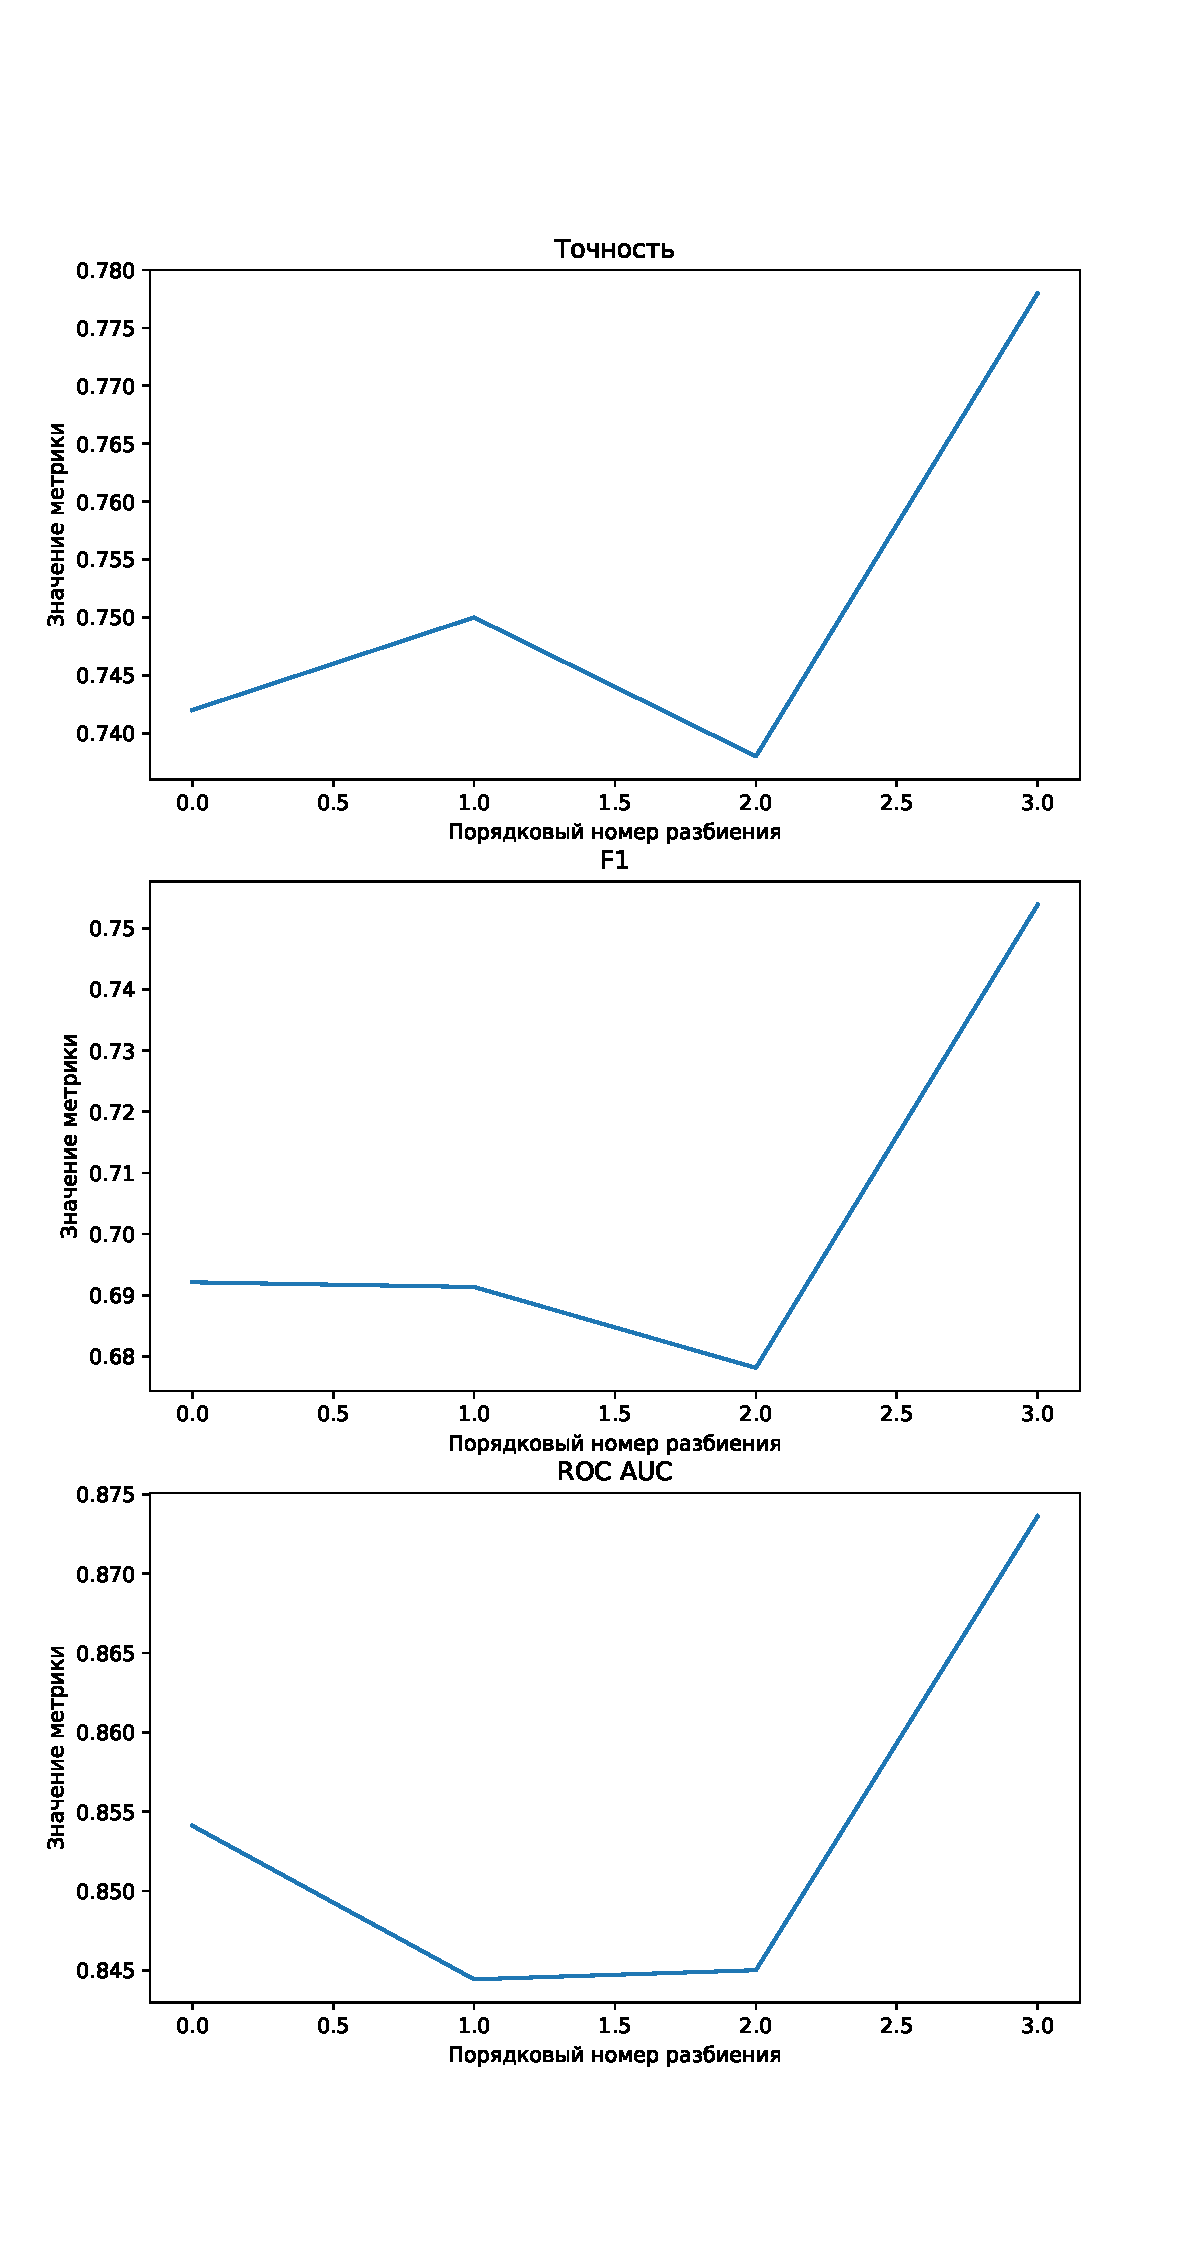
\includegraphics[height=23cm]{inc/plots/knnMetricsBag.pdf}
	\caption{ Оценки классификатора в зависимости от номера разбиения, полученные с использованием метода K-ближайших соседей (метод векторизации --  ``мешок слов''). }
	\label{img:knnMetricsBag}
\end{figure}


Параметры модели при применении векторизации BERT:
\begin{itemize}
	\item скорость обучения -- ;
\end{itemize}

На рисунке \ref{img:knnMatrBert} представлены матрицы ошибок, полученные с использованием метода K-ближайших соседей, метод векторизации -- BERT.
\begin{figure}[H]
	\centering
	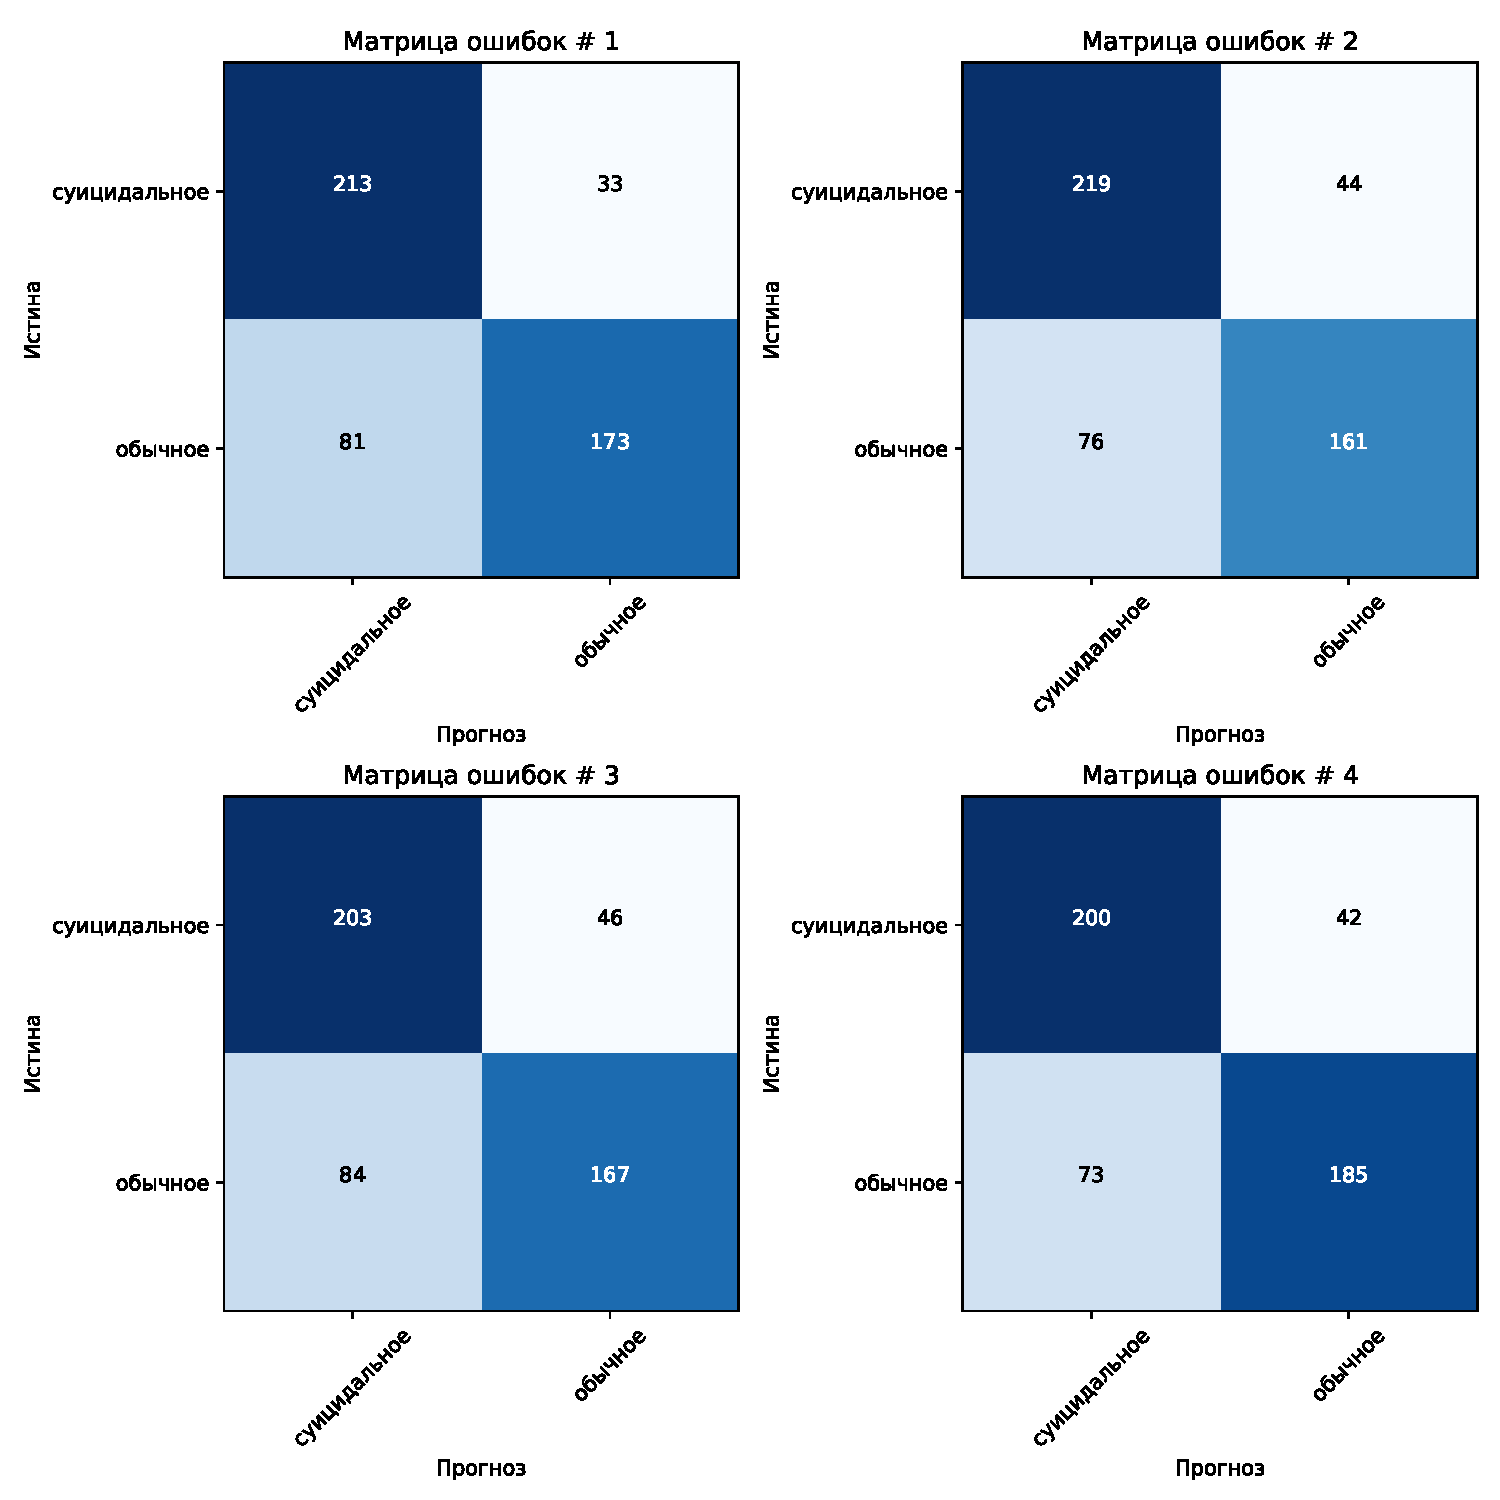
\includegraphics[width=\textwidth]{inc/plots/knnMatrBert.pdf}
	\caption{ Матрицы ошибок в зависимости от номера разбиения, полученные с использованием метода K-ближайших соседей (метод векторизации -- BERT). }
	\label{img:knnMatrBert}
\end{figure}

На рисунке \ref{img:knnMetricsBert} представлены оценки классификатора, полученные с использованием метода K-ближайших соседей, метод векторизации -- BERT.
\begin{figure}[H]
	\centering
	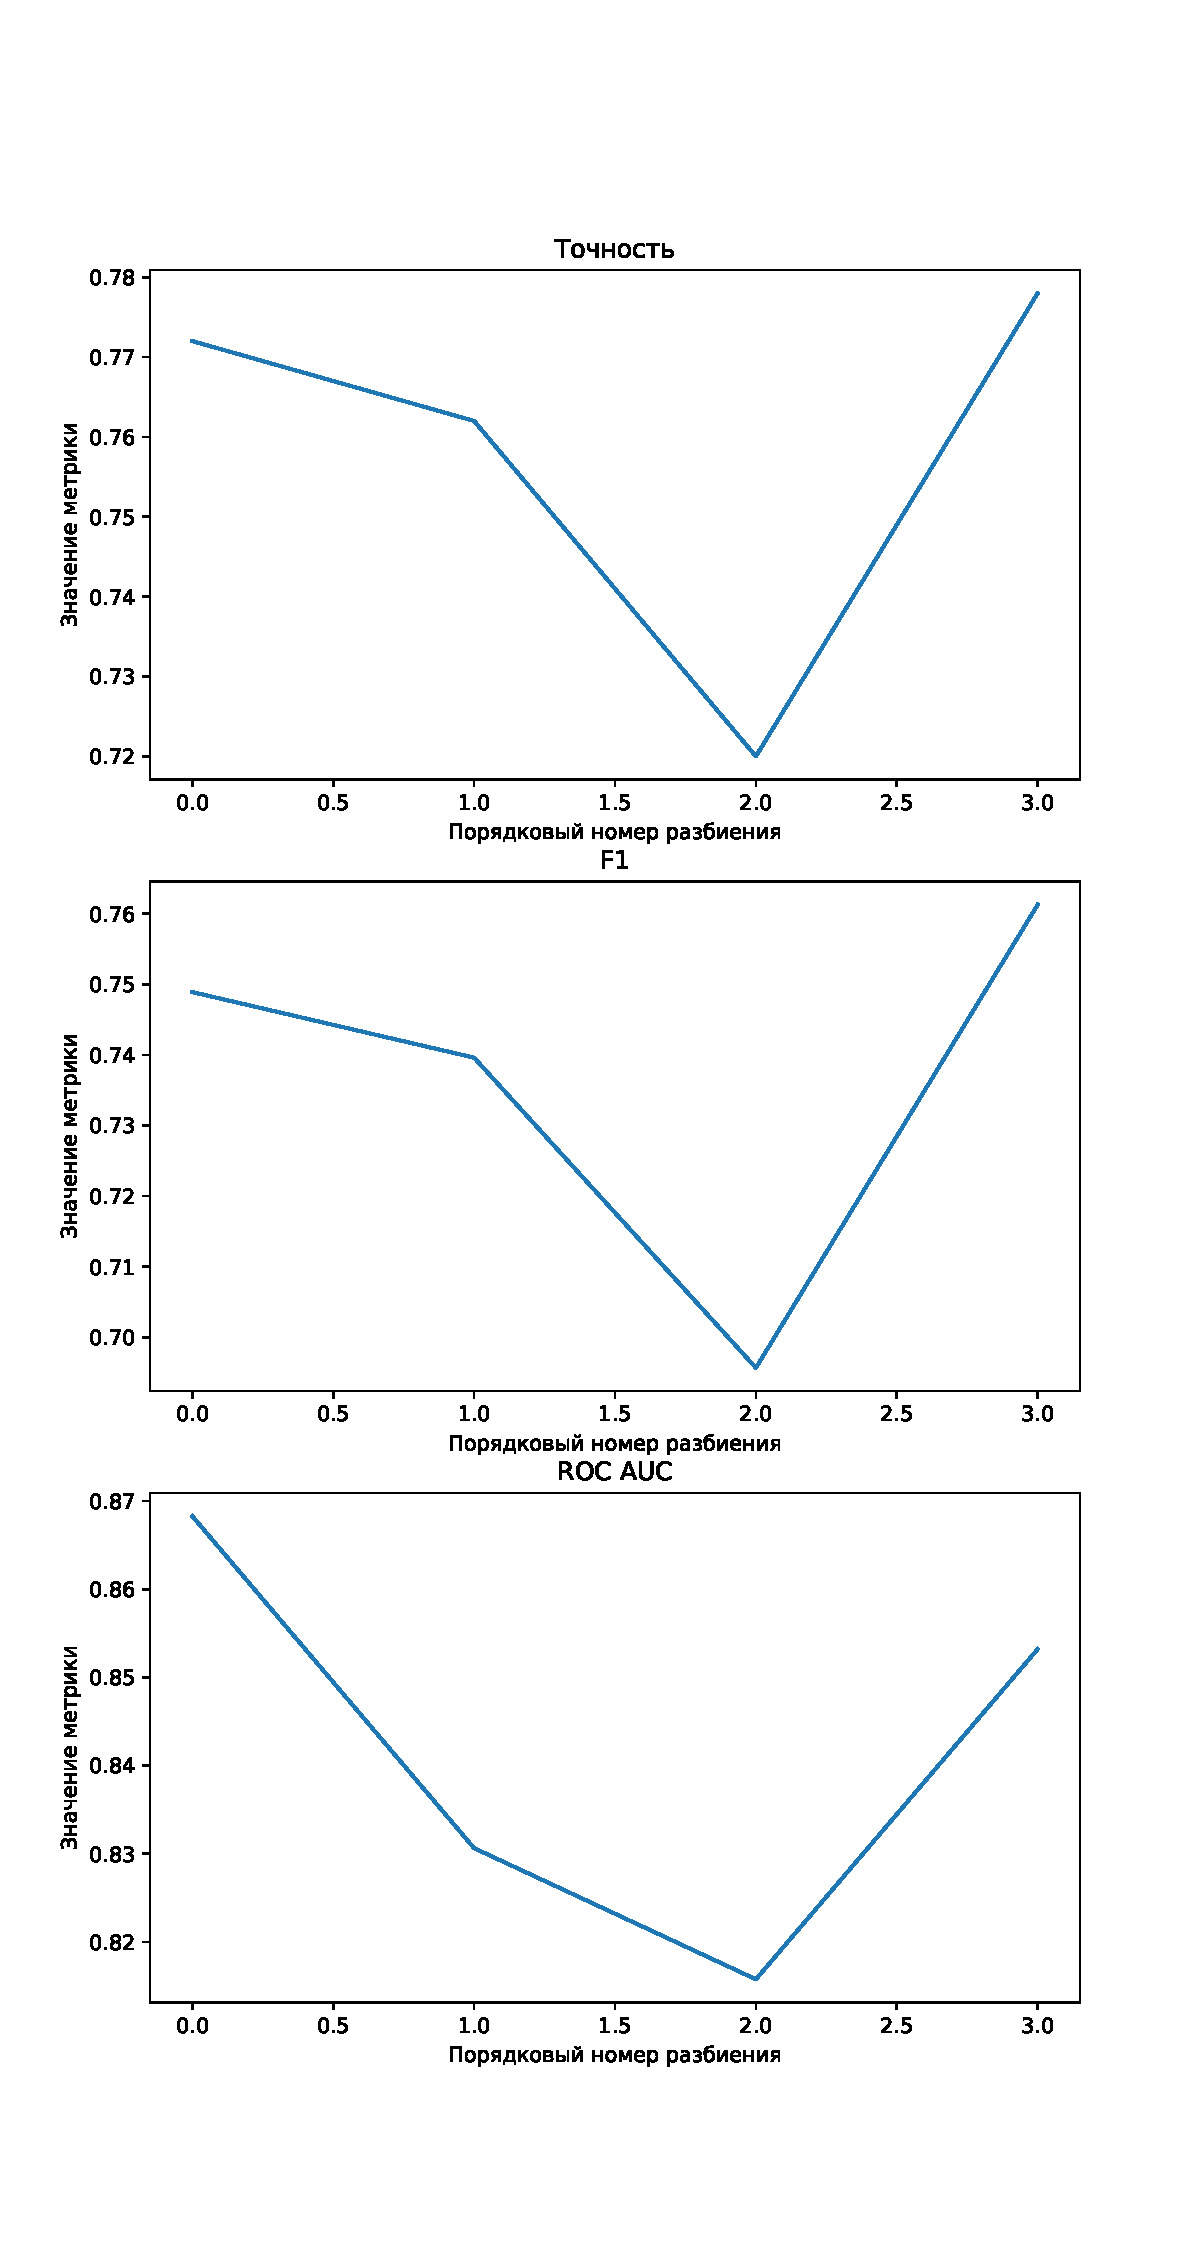
\includegraphics[height=23cm]{inc/plots/knnMetricsBert.pdf}
	\caption{ Оценки классификатора в зависимости от номера разбиения, полученные с использованием метода K-ближайших соседей (метод векторизации -- BERT). }
	\label{img:knnMetricsBert}
\end{figure}



\subsection{ Логистическая регрессия }

Параметры модели при применении метода векторизации ``мешок слов'':
\begin{itemize}
	\item скорость обучения -- ;
\end{itemize}

На рисунке \ref{img:logicMatrBag} представлены матрицы ошибок, полученные с использованием логистической регрессии, метод векторизации -- ``мешок слов''.
\begin{figure}[H]
	\centering
	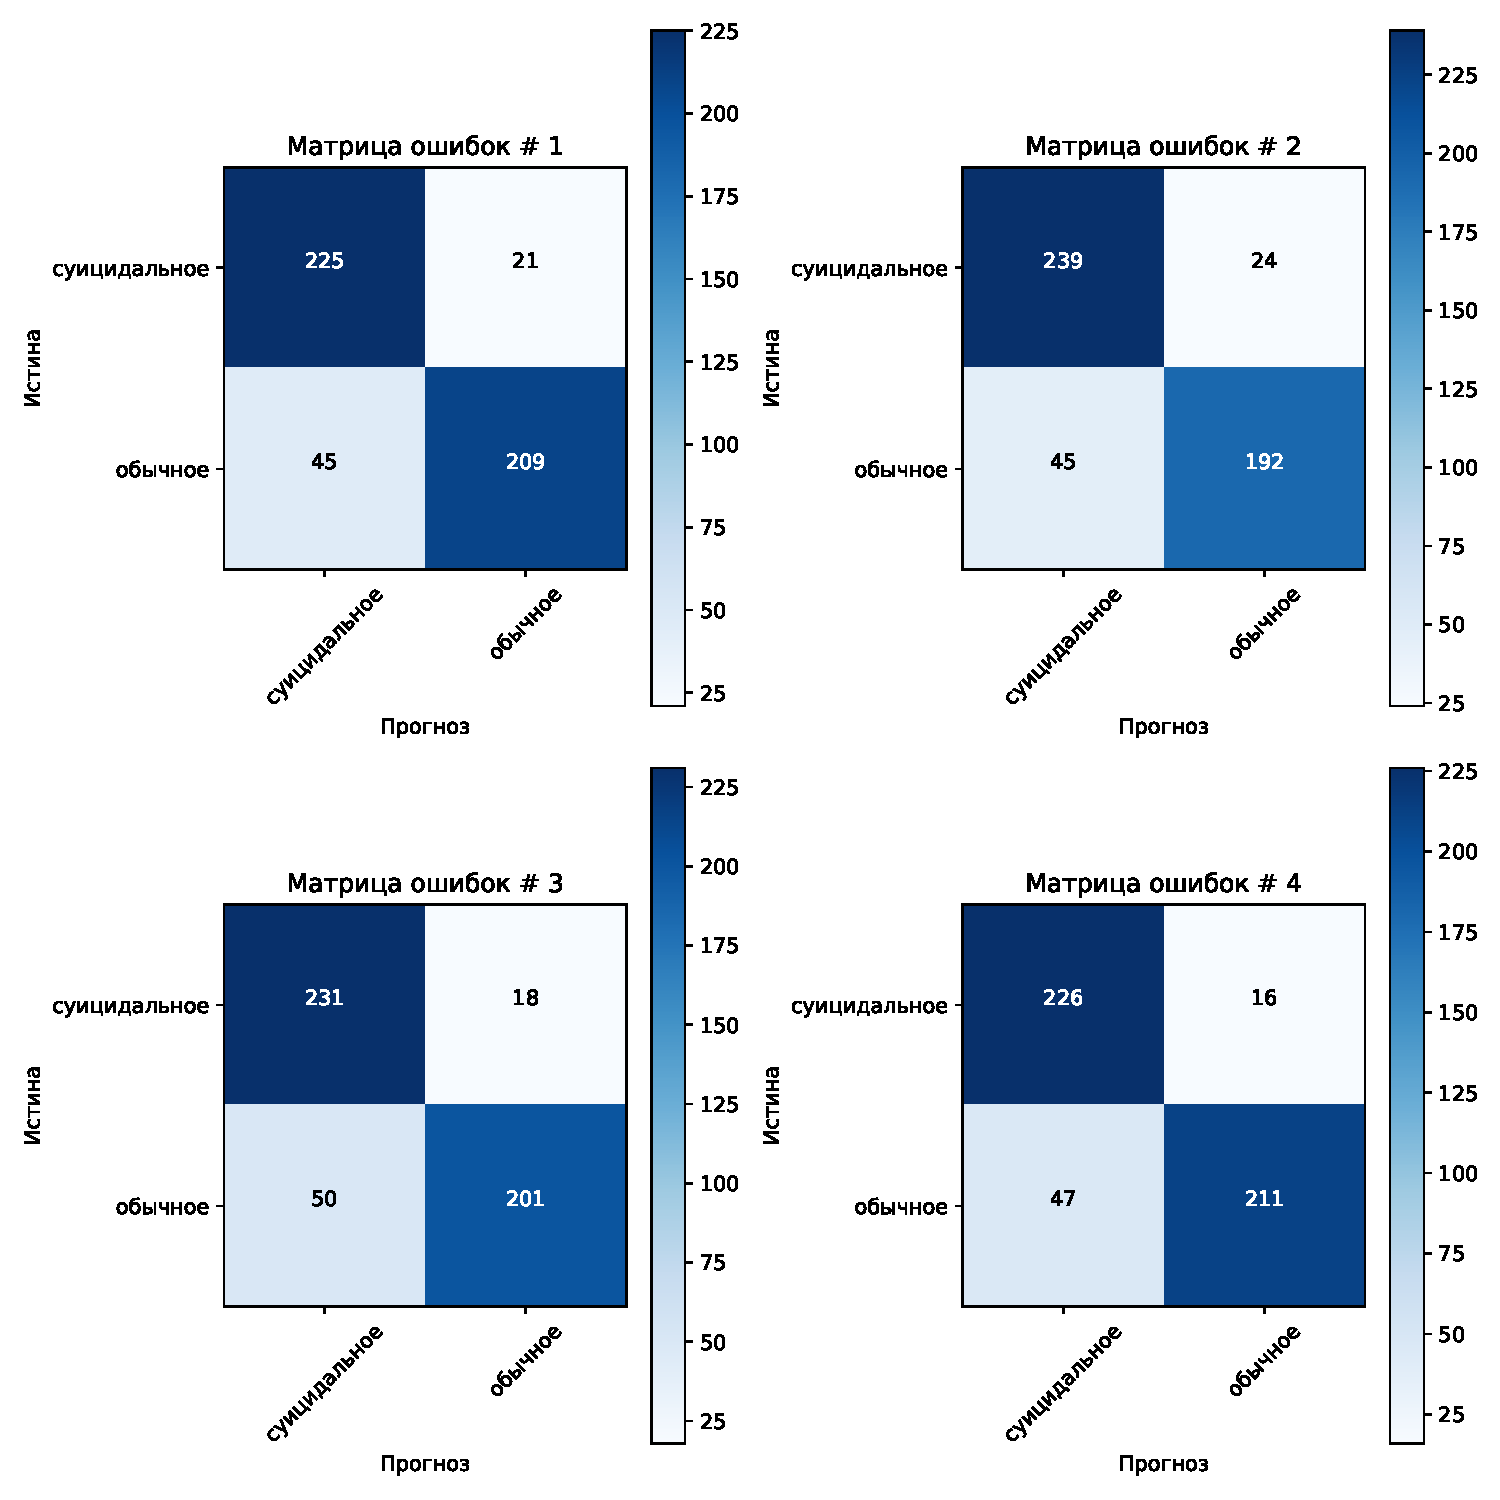
\includegraphics[width=\textwidth]{inc/plots/logicMatrBag.pdf}
	\caption{ Матрицы ошибок в зависимости от номера разбиения, полученные с использованием логистической регрессии (метод векторизации -- ``мешок слов''). }
	\label{img:logicMatrBag}
\end{figure}

На рисунке \ref{img:logicMetricsBag} представлены оценки классификатора, полученные с использованием логистической регрессии, метод векторизации -- ``мешок слов''.
\begin{figure}[H]
	\centering
	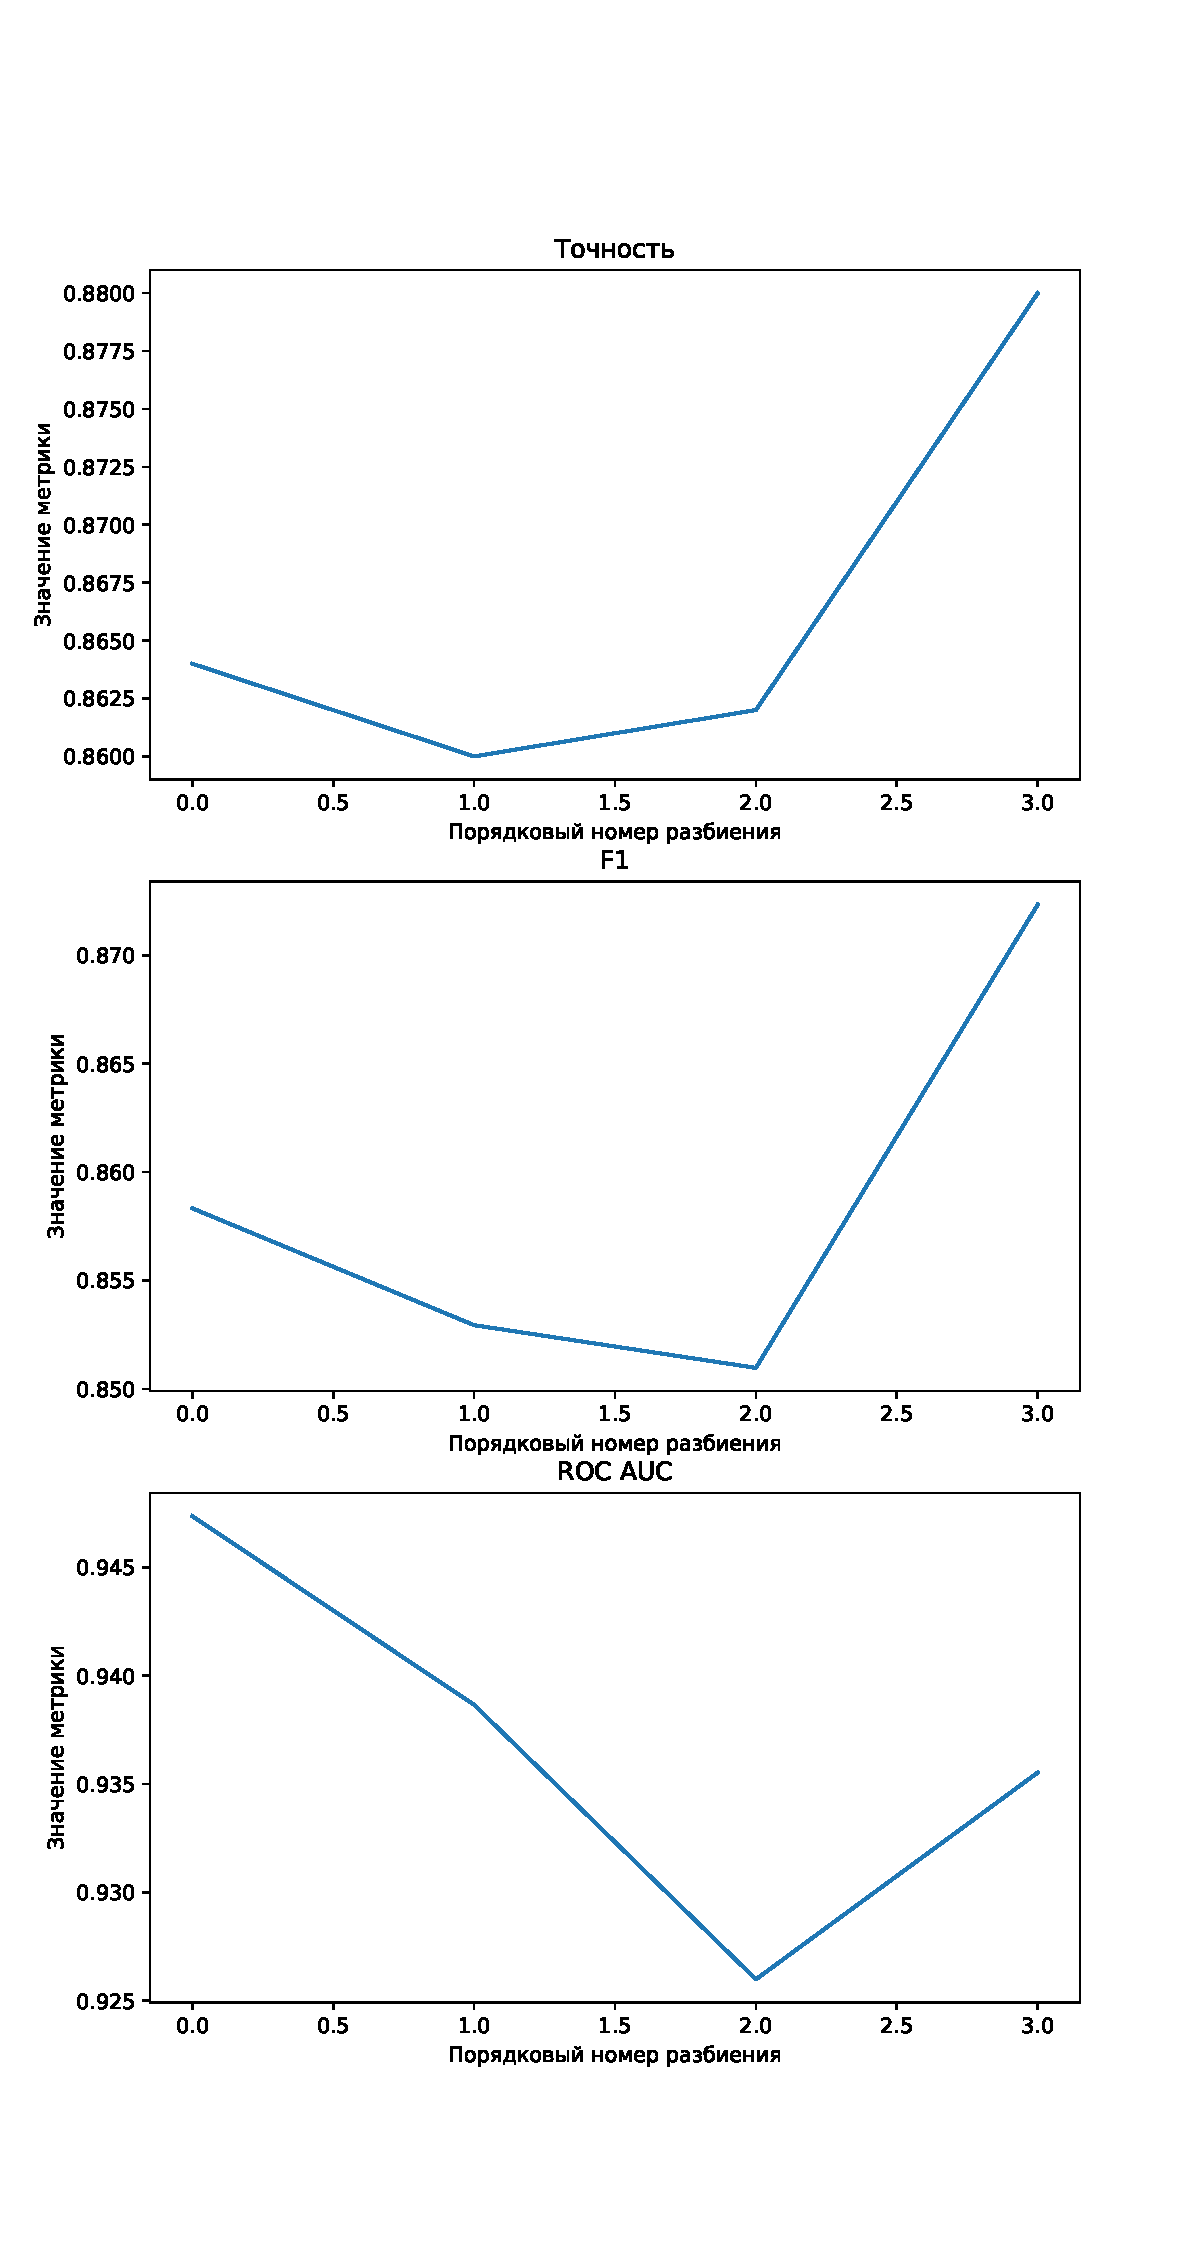
\includegraphics[height=23cm]{inc/plots/logicMetricsBag.pdf}
	\caption{ Оценки классификатора в зависимости от номера разбиения, полученные с использованием логистической регрессии (метод векторизации --  ``мешок слов''). }
	\label{img:logicMetricsBag}
\end{figure}


Параметры модели при применении векторизации BERT:
\begin{itemize}
	\item скорость обучения -- ;
\end{itemize}
На рисунке \ref{img:logicMatrBert} представлены матрицы ошибок, полученные с использованием логистической регрессии, метод векторизации -- BERT.

\begin{figure}[H]
	\centering
	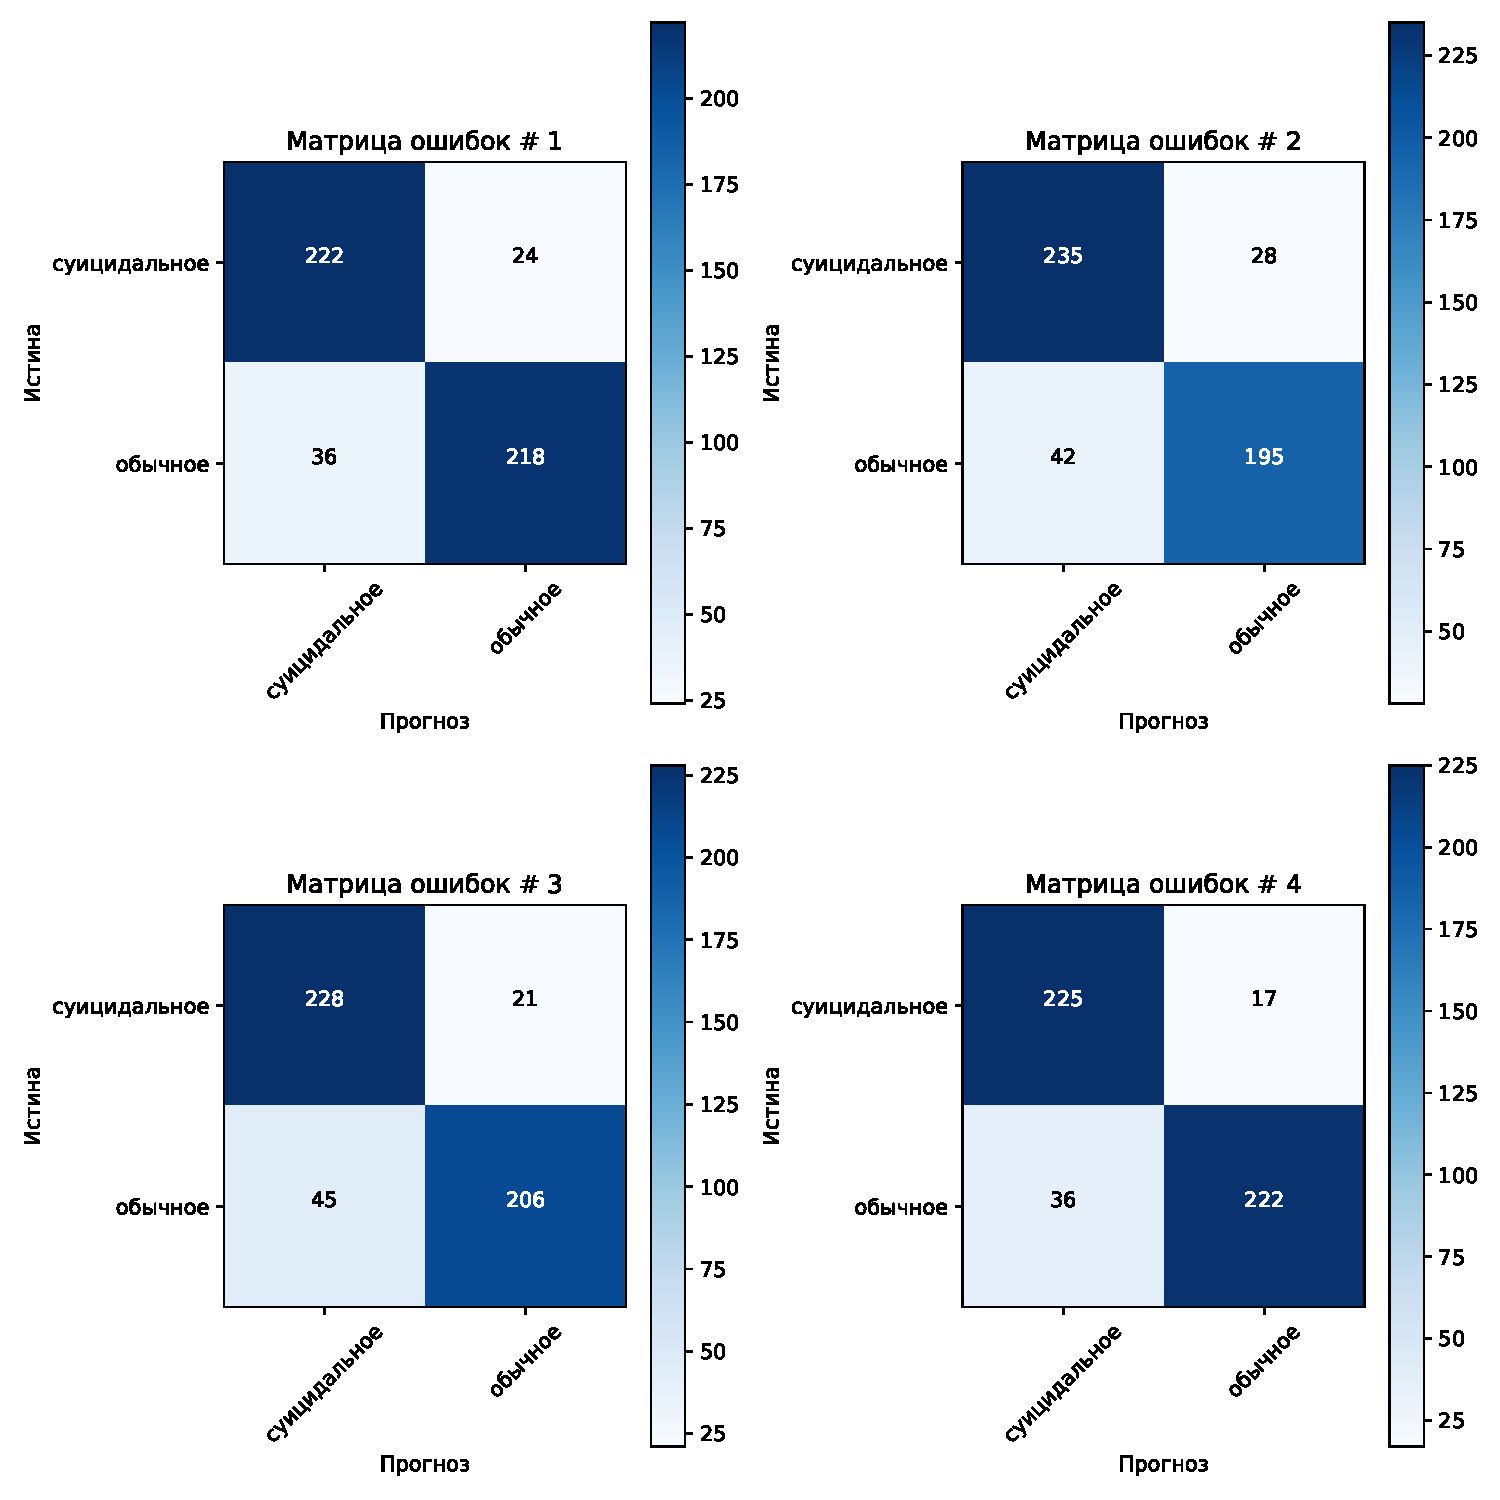
\includegraphics[width=\textwidth]{inc/plots/logicMatrBert.pdf}
	\caption{ Матрицы ошибок в зависимости от номера разбиения, полученные с использованием логистической регрессии (метод векторизации -- BERT). }
	\label{img:logicMatrBert}
\end{figure}

На рисунке \ref{img:logicMetricsBert} представлены оценки классификатора, полученные с использованием логистической регрессии, метод векторизации -- BERT.
\begin{figure}[H]
	\centering
	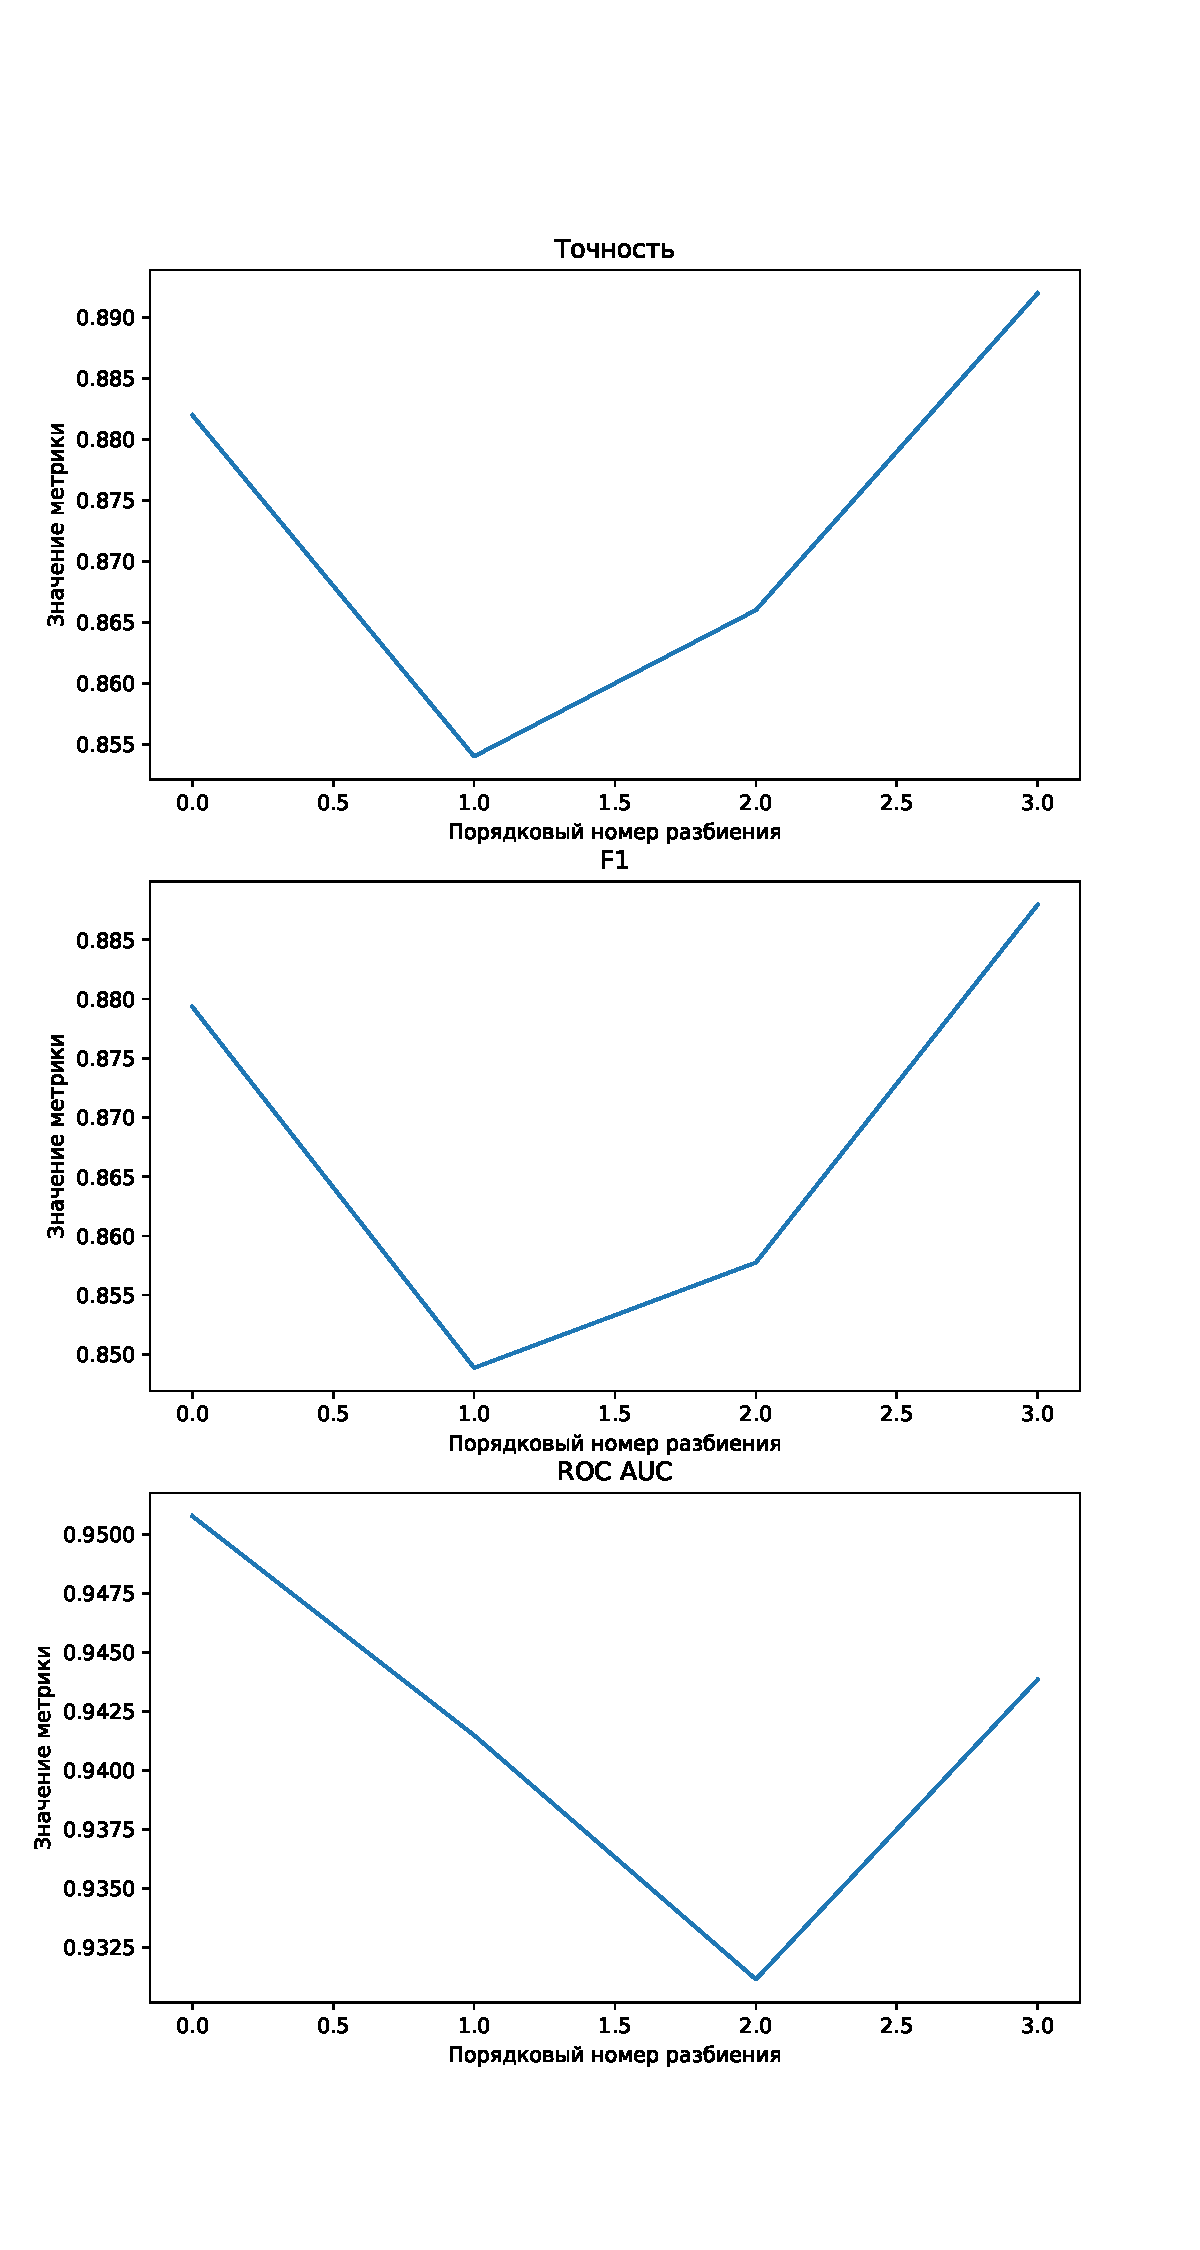
\includegraphics[height=23cm]{inc/plots/logicMetricsBert.pdf}
	\caption{ Оценки классификатора в зависимости от номера разбиения, полученные с использованием логистической регрессии (метод векторизации -- BERT). }
	\label{img:logicMetricsBert}
\end{figure}



\subsection{ Перцептрон }

Параметры модели при применении метода векторизации ``мешок слов'':
\begin{itemize}
	\item скорость обучения -- ;
\end{itemize}

На рисунке \ref{img:perceptronMatrBag} представлены матрицы ошибок, полученные с использованием перцептрона, метод векторизации -- ``мешок слов''.
\begin{figure}[H]
	\centering
	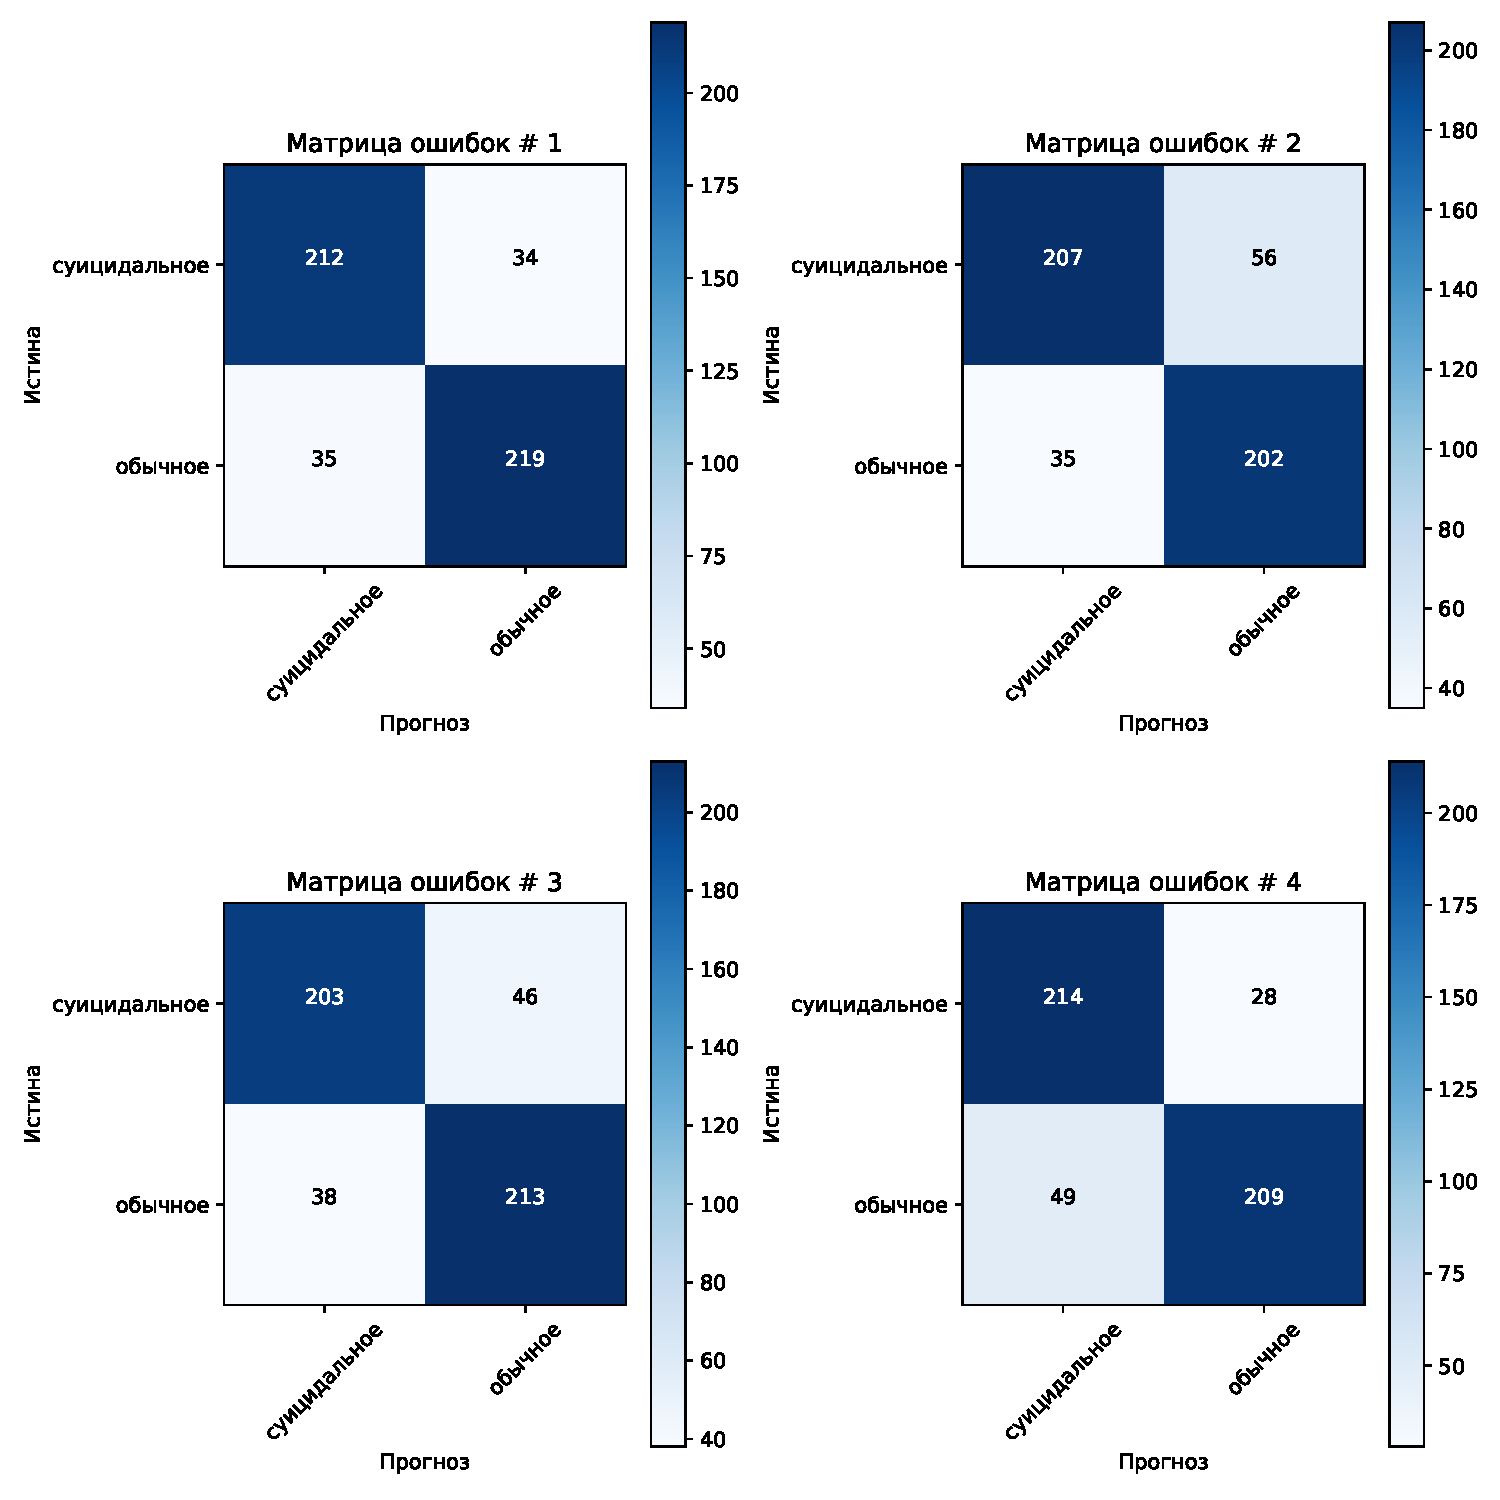
\includegraphics[width=\textwidth]{inc/plots/perceptronMatrBag.pdf}
	\caption{ Матрицы ошибок в зависимости от номера разбиения, полученные с использованием перцептрона (метод векторизации -- ``мешок слов''). }
	\label{img:perceptronMatrBag}
\end{figure}

На рисунке \ref{img:perceptronMetricsBag} представлены оценки классификатора, полученные с использованием перцептрона, метод векторизации -- ``мешок слов''.
\begin{figure}[H]
	\centering
	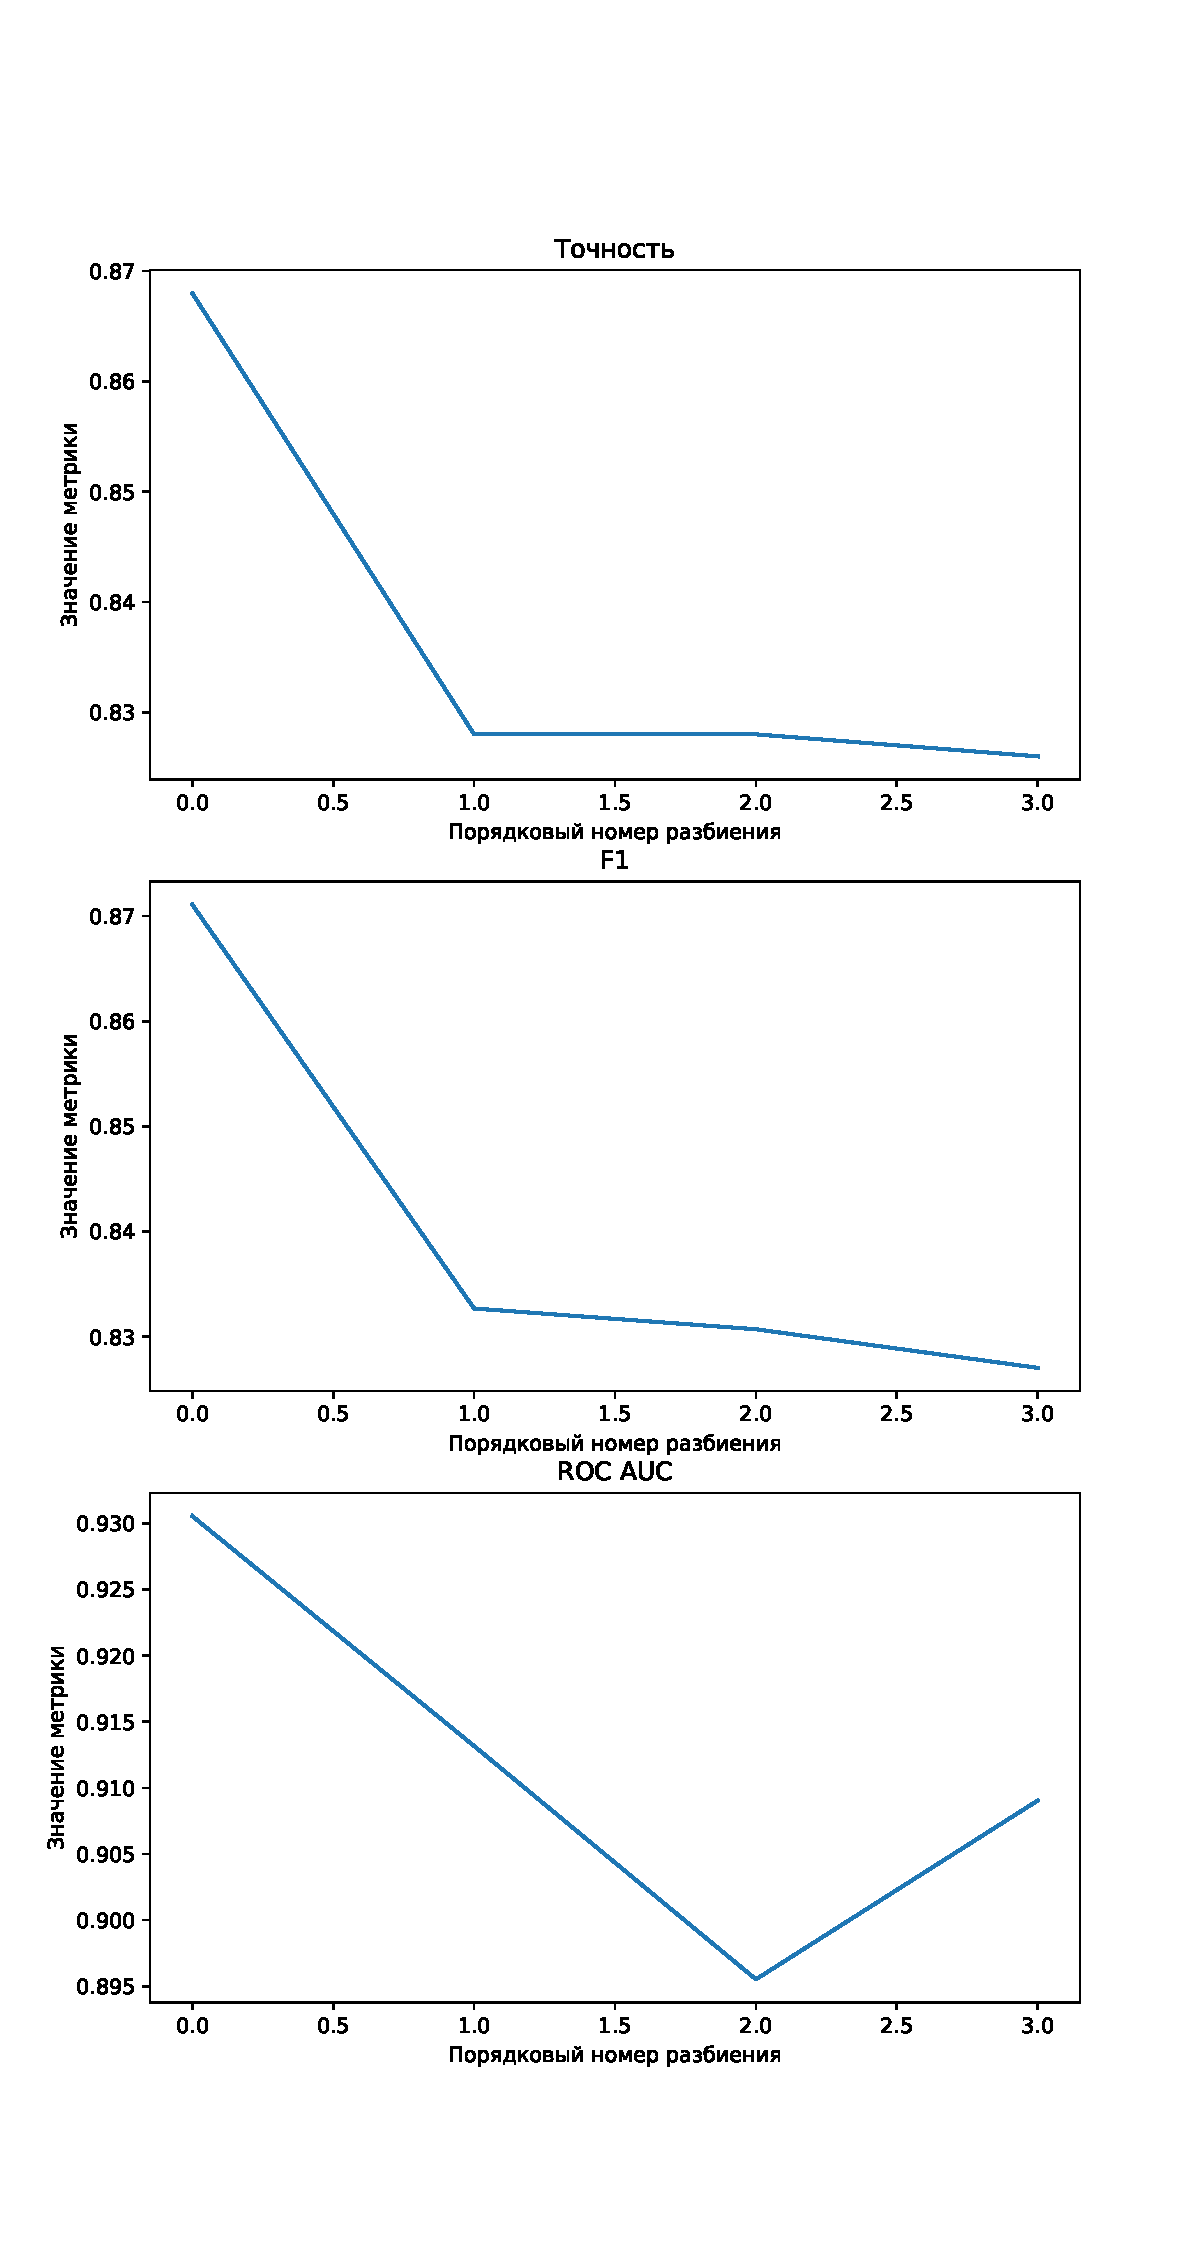
\includegraphics[height=23cm]{inc/plots/perceptronMetricsBag.pdf}
	\caption{ Оценки классификатора в зависимости от номера разбиения, полученные с использованием перцептрона (метод векторизации --  ``мешок слов''). }
	\label{img:perceptronMetricsBag}
\end{figure}


Параметры модели при применении векторизации BERT:
\begin{itemize}
	\item скорость обучения -- ;
\end{itemize}

На рисунке \ref{img:perceptronMatrBert} представлены матрицы ошибок, полученные с использованием перцептрона, метод векторизации -- BERT.
\begin{figure}[H]
	\centering
	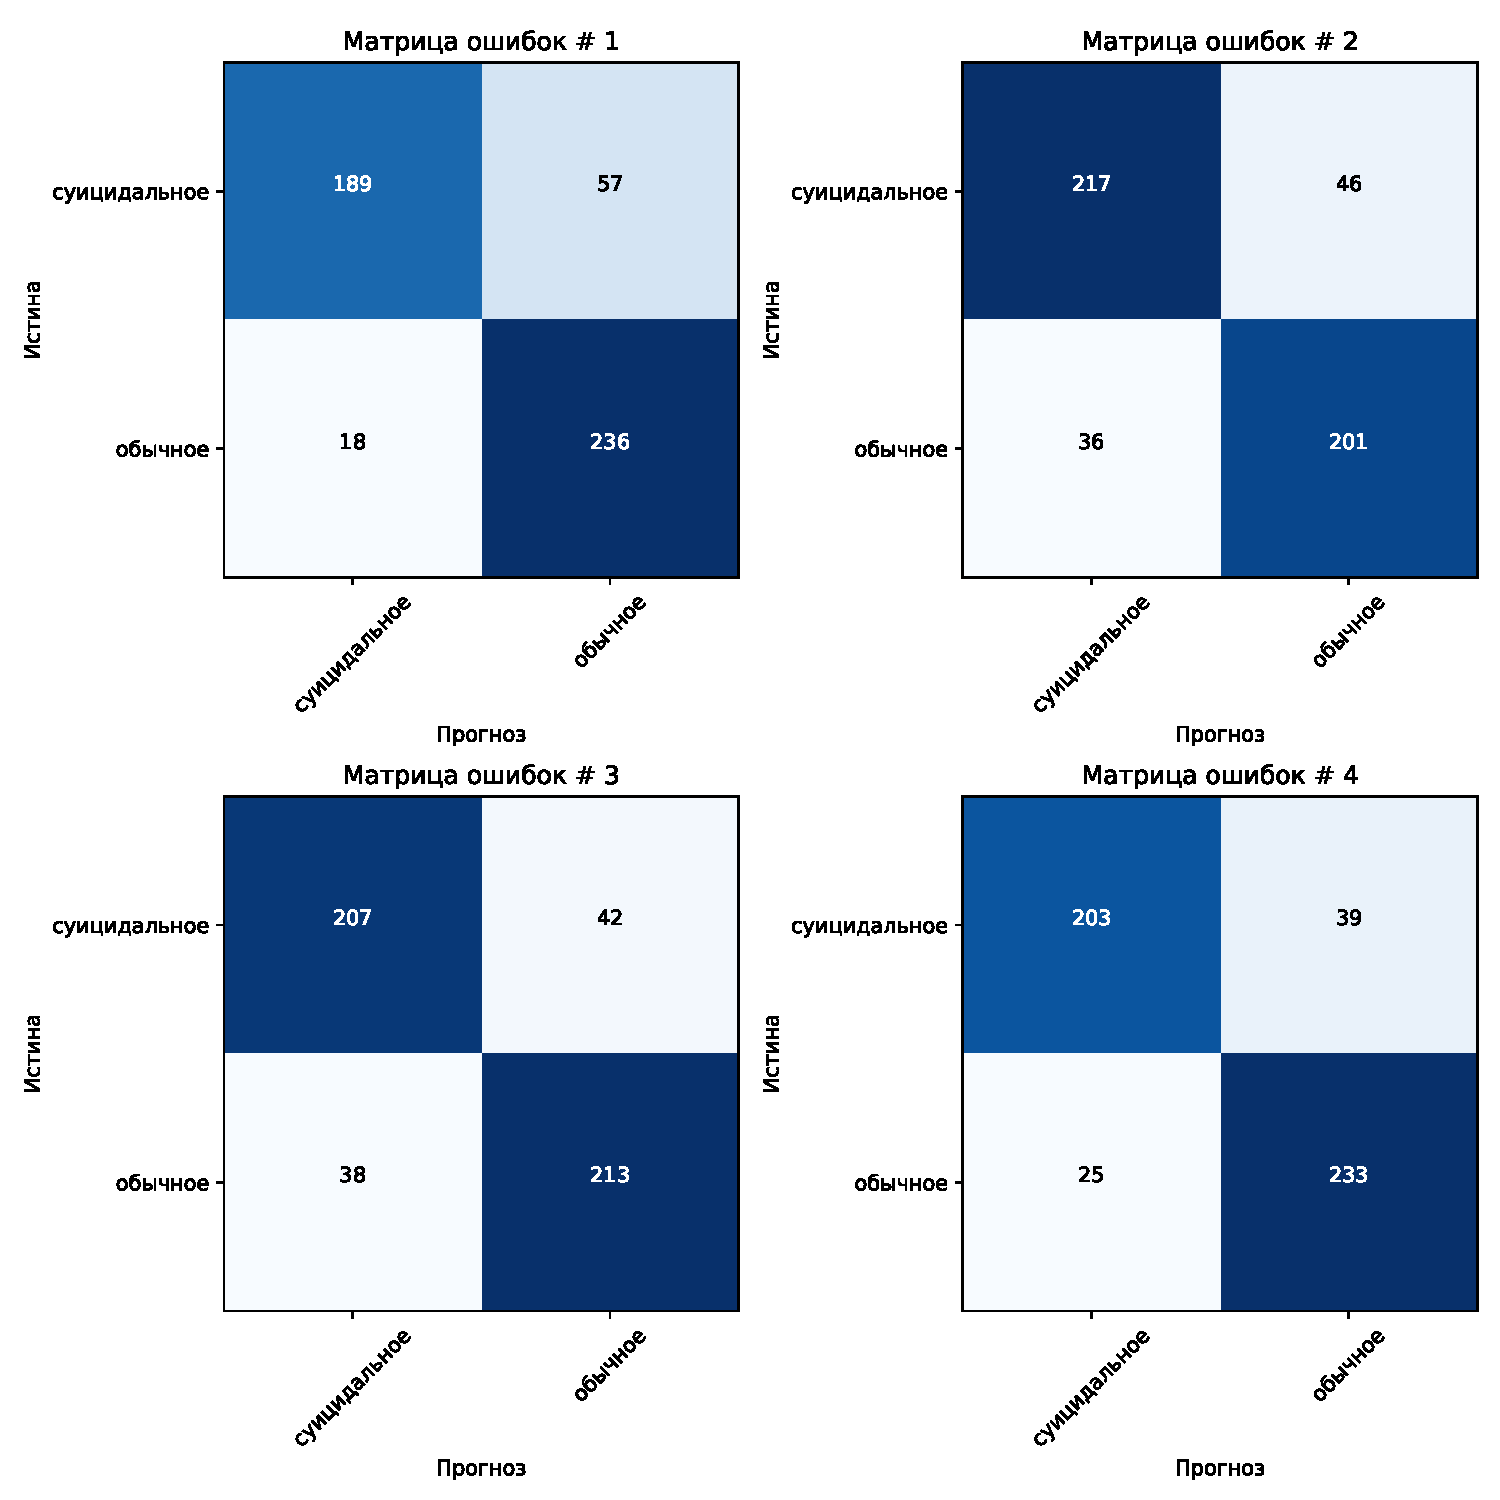
\includegraphics[width=\textwidth]{inc/plots/perceptronMatrBert.pdf}
	\caption{ Матрицы ошибок в зависимости от номера разбиения, полученные с использованием перцептрона (метод векторизации -- BERT). }
	\label{img:perceptronMatrBert}
\end{figure}

На рисунке \ref{img:perceptronMetricsBert} представлены оценки классификатора, полученные с использованием перцептрона, метод векторизации -- BERT.
\begin{figure}[H]
	\centering
	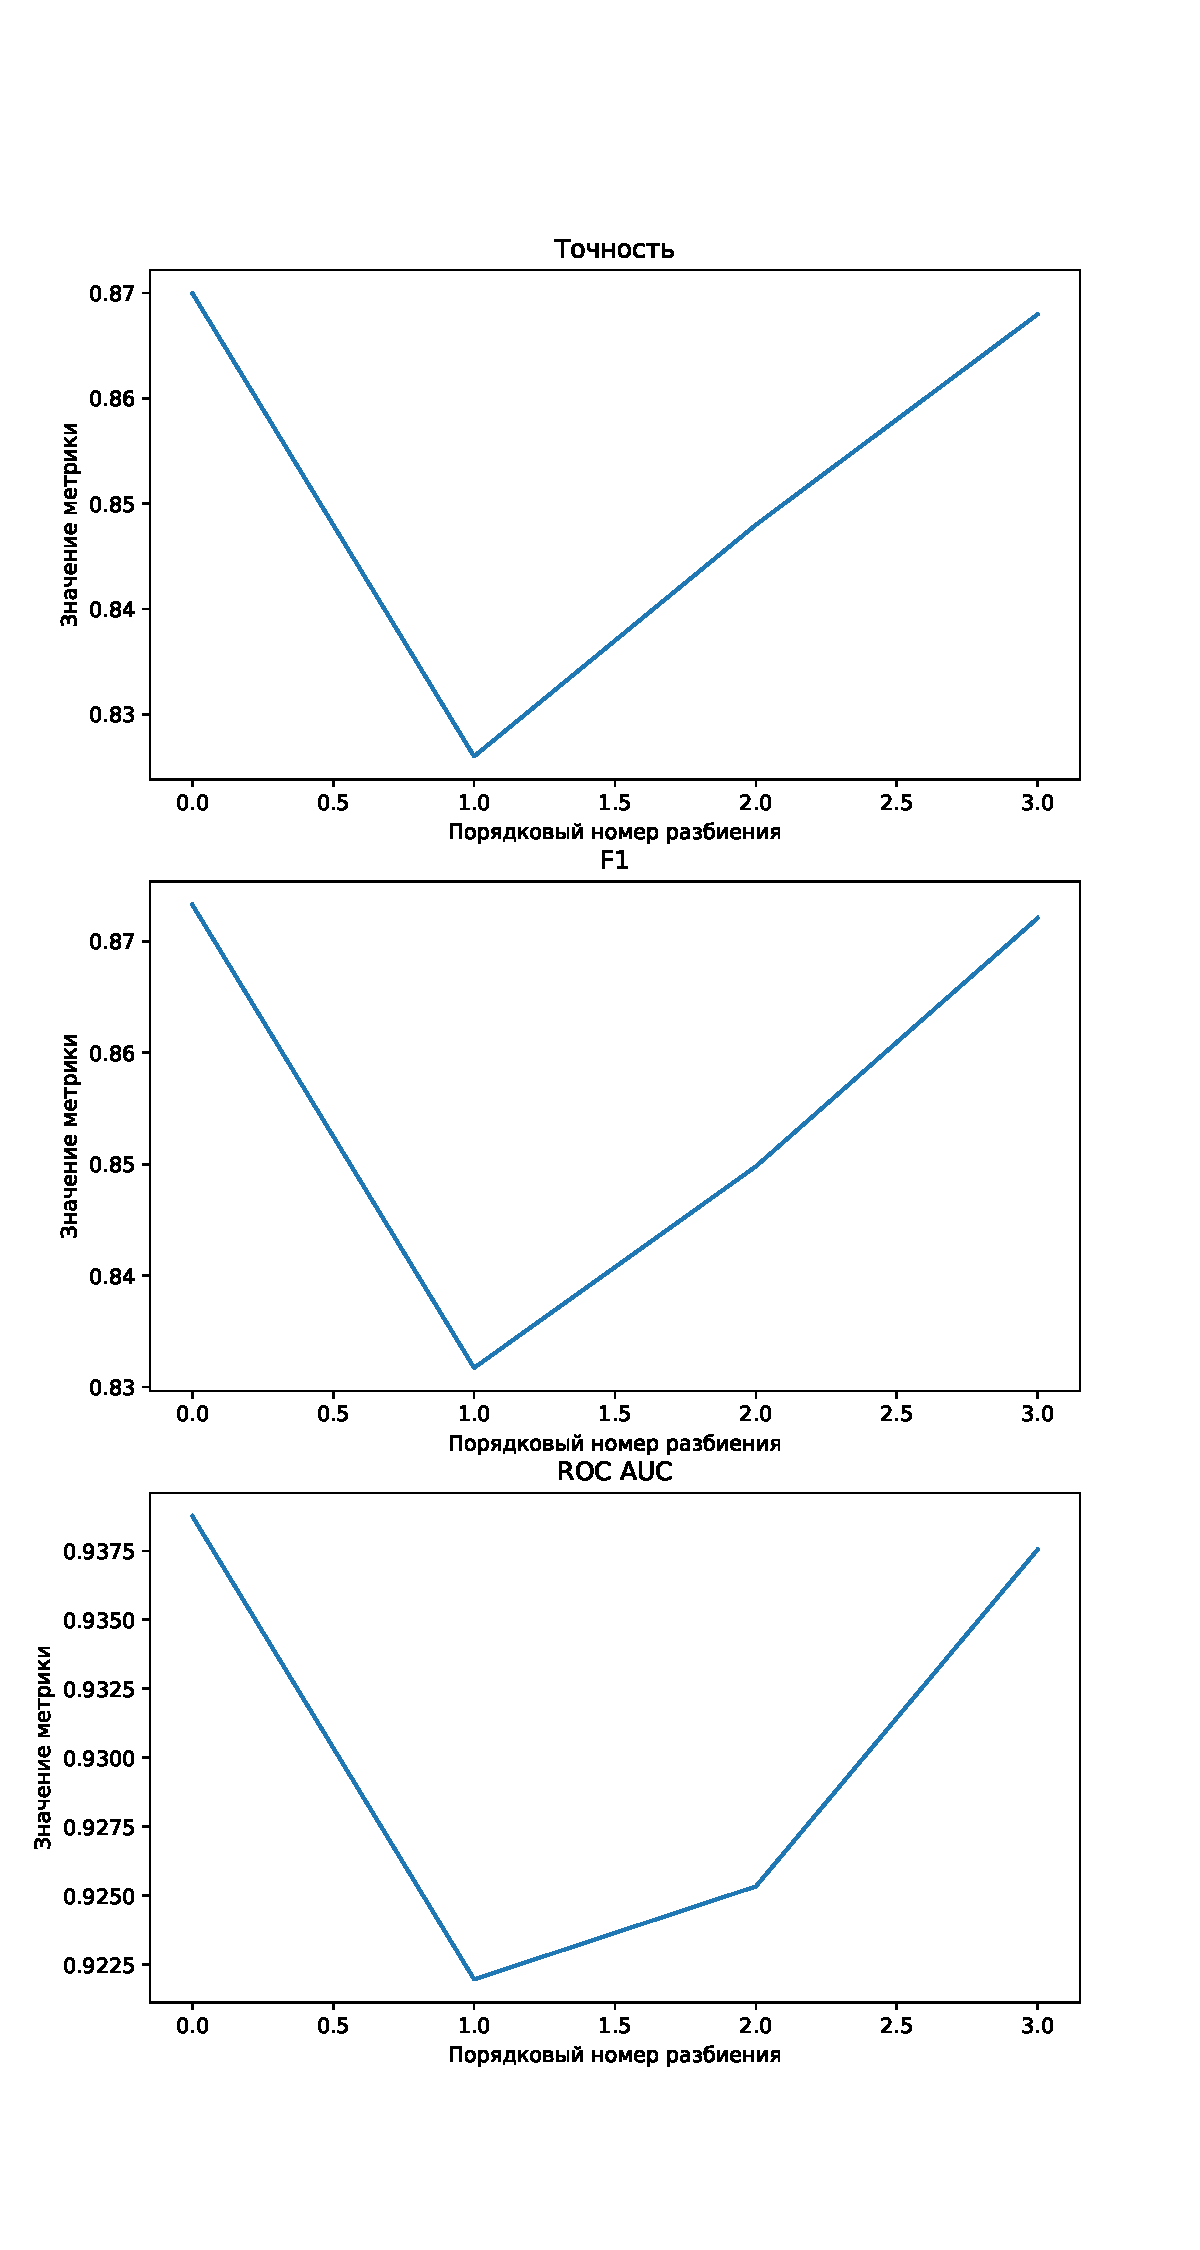
\includegraphics[height=23cm]{inc/plots/perceptronMetricsBert.pdf}
	\caption{ Оценки классификатора в зависимости от номера разбиения, полученные с использованием перцептрона (метод векторизации -- BERT). }
	\label{img:perceptronMetricsBert}
\end{figure}

\subsection{ Результат }

Таблица
